% lancement avec sweave, xelatex et biber
%%%%%%%%%%%%%%%%%%%%%%%%%%%%%%%%%%%%%%%%%%%%%%%%%%%%%%%%%%%%%%%%%%%%%%%%%%%%
%%
%%============================================================
%% DOCUMENT CLASS SETUP
%%============================================================
%%
\documentclass[11pt,twocolumn,titlepage,twoside]{article}
\setlength{\columnsep}{0.8cm} % séparateur central
\usepackage{float}
\usepackage[section]{placeins}  %The placeins package provides the command \FloatBarrier

%%============================================================
%%============================================================
%% PACKAGE SETUP
\usepackage{Sweave}
%\SweaveOpts{pdf=TRUE, echo=FALSE, fig=FALSE, eps=FALSE, tidy=T, width=4,
%height=4, keep.source=TRUE}

%% Input and language packages.
%\usepackage[utf8]{inputenc} %encodage du fichier source not used with xelatex
\usepackage[T1]{fontenc}  %gestion des accents (pour les pdf) 
%\usepackage[english]{babel}
\usepackage[francais]{babel}
\usepackage{dirtytalk} % pour les guillemet \say{ceci sera quoté  et \say{nested quote}}
%https://tex.stackexchange.com/questions/464585/what-tips-and-tricks-should-i-know-when-using-the-georgia-font-in-latex/464586
% \usepackage{fontspec} % charte graphique EPTB
\usepackage{amsmath}
\usepackage[math-style=ISO]{unicode-math}
\usepackage{microtype}
\defaultfontfeatures{Scale=MatchLowercase}
\setmainfont{Georgia}[Scale = 1.0]
\setmathfont{Asana Math.otf}
\addto\captionsfrench{\def\tablename{Tableau}}
\addto\captionsfrench{\renewcommand*{\contentsname}{Sommaire:}}
\addto{\captionsfrench}{\renewcommand*{\abstractname}{Résumé}}
\addto{\captionsfrench}{\renewcommand*{\listfigurename}{Figures}}
\addto{\captionsfrench}{\renewcommand*{\listtablename}{Tableaux}}

%% Parskip is the extra vertical space inserted before a paragraph. It has a natural length of zero but should be a rubber length so that it may be stretched in a flushbottom environment. To increase \parskip to skip a line between paragraphs one could use \addtolength{\parskip} {\baselineskip}.
\usepackage{parskip}

%% Sets space between lines.
\usepackage{setspace} 


%% If you use PostScript figures in your article
%% use the graphics package for simple commands
%\usepackage{graphics}
%% or use the graphicx package for more complicated commands (places the float at precisely the location in the LaTeX code [H]).
\usepackage{graphicx} 
\usepackage{float}
%% or use the epsfig package if you prefer to use the old commands.
%\usepackage{epsfig}

%% Using captions in floating environment. Note: might not work with other packages.
%\usepackage{caption}

%% Making numbered and bulleted lists.
\usepackage{enumerate}
\usepackage{enumitem} % listes avec A B C
%\definecolor{marron}{rgb}{0.64,0.16,0.16}
%% Math packages
%\usepackage{amsmath, amssymb}

%% The amsthm package provides extended theorem environments.
%\usepackage{amsthm}

%% The verbatim environment, \begin{verbatim} ... \end{verbatim}, permits us to insert large sections of reformatted text in a LaTeX file (including block of comments). It is very handy for inserting large chunks of code in a document, for example, literal TeX code or the Maple code you sweated over and now want to comment on.
%\usepackage{verbatim}

%% Add hyperlinks, so that you can click on references, theorem numbers etc. to jump to the place where they are in the paper (at least for the DVI and PDF versions), it seems that \documentclass{article} does not work with hyperref; use instead \documentclass{amsart}. Note: first test it with Elsevier template!

\usepackage[usenames,dvipsnames,svgnames,table]{xcolor} % Invoke the package with the usenames and dvipsnames option to get 68 colors
\usepackage{color}
\definecolor{bleu_EV}{RGB}{0,33,143}
\definecolor{turquoise_EV}{RGB}{0,201,196}
\definecolor{orange_EV}{RGB}{255,117,87}
\definecolor{orange_EVf}{RGB}{178,81,60}
\definecolor{bleu_clair_EV}{RGB}{51,181,255}
\definecolor{jaune_EV}{RGB}{255,180,40}

\definecolor{grisbleu}{RGB}{66,66,143}
\definecolor{grisbleufonce}{RGB}{21,21,93}
\definecolor{rouille}{RGB}{135,71,45}
\definecolor{orange}{RGB}{255,165,0}
\definecolor{turquoise}{RGB}{0,128,128}
\definecolor{limegreen}{RGB}{50,205,50} % correspond a limegreen en R
\definecolor{purple2}{RGB}{160,32,240}
\definecolor{purplesombre}{RGB}{50,0,74}
\definecolor{purplemedian}{RGB}{67,0,100}
\definecolor{purpleclair}{RGB}{115,0,171}
\definecolor{violetred}{RGB}{208,32,144}
% A EDITER LIGNE 726 dans elsarticle.cls

%% The numcompress package shorten the last page in references.
%% `nodots' option removes dots from firstnames in references.
%\usepackage[nodots]{numcompress}

%% The lineno packages adds line numbers. Start line numbering with
%% \begin{linenumbers}, end it with \end{linenumbers}. Or switch it on
%% for the whole article with \linenumbers after \end{frontmatter}.
%% \usepackage{lineno}

%% If you are printing how many pages you submitted...
%\usepackage{lastpage}

%% The \url{...} command does all the work: It sets the enclosed expression in the appropriate typewriter style font, it takes care of any necessary linebreaking, and it chooses break points intelligently (e.g., between components of an address), and it ensures that special symbols such as the tilde symbol or the "at" symbol get typeset correctly.
\usepackage{url}

%% A new implementation of LATEX's tabular and array environment.
\usepackage{array}
\usepackage{enumerate}
\usepackage{longtable}
\usepackage{multirow}
\usepackage{siunitx,booktabs}
\sisetup{group-separator={~}, 
group-minimum-digits={3}, % 3 caractères pour séparer les
output-decimal-marker={.}, % separateur
round-mode = places, % nombre de décimales après la virgule
round-precision = 0 % precision des arrondis
}
\usepackage{caption} % pour les subfigures http://en.wikibooks.org/wiki/LaTeX/Floats,_Figures_and_Captions
\usepackage{subcaption} % pour les subfigures

\addto{\captionsfrench}{\renewcommand{\tablename}{Tableau}}
\usepackage{calc}
\newlength\defaultparindent
\setlength{\defaultparindent}{\parindent}   %save default indentation   
%http://tex.stackexchange.com/questions/59175/boxes-overflow-column
%%============================================================
%% BIBLIOGRAPHY SETUP
%%============================================================
\usepackage[style=authoryear, %numeric
            natbib=true, % citep and citet
            backend=biber, % default for biblatex
            bibencoding=utf8,
            url=false, 
            doi=false,
            firstinits=true, % pas de prenoms
            %sorting=nyt, % name, year, title
            eprint=false]{biblatex} % option natbib to use cite and citep
\addbibresource{didson2023.bib}
%\usepackage[round, comma, sort]{natbib}


%% natbib.sty is loaded by default. However, natbib options can be
%% provided with \biboptions{...} command. Following options are
%% valid:

%%   round  -  round parentheses are used (default)
%%   square -  square brackets are used   [option]
%%   curly  -  curly braces are used      {option}
%%   angle  -  angle brackets are used    <option>
%%   semicolon  -  multiple citations separated by semi-colon (default)
%%   colon  - same as semicolon, an earlier confusion
%%   comma  -  separated by comma
%%   authoryear - selects author-year citations (default)
%%   numbers-  selects numerical citations
%%   super  -  numerical citations as superscripts
%%   sort   -  sorts multiple citations according to order in ref. list
%%   sort&compress   -  like sort, but also compresses numerical citations
%%   compress - compresses without sorting
%%   longnamesfirst  -  makes first citation full author list
%%
%%  e.g. \biboptions{longnamesfirst,comma}

\usepackage{hyperref}
\hypersetup{
     colorlinks=true,
     linkcolor=orange_EVf,
     urlcolor=bleu_EV,
     citecolor=grisbleufonce,
     bookmarks=true,  %créé des signets pour Acrobat
     bookmarksopen=true,            %si les signets Acrobat sont créés,
                                    %les afficher complètement.
     pdftitle={Suivi de la dévalaison de l'anguille argentée en 2022--2023
     (11ème année) sur la Vilaine à l'aide d'un didson},
     %informations apparaissant dans
     pdfauthor={Cédric Briand,Brice Sauvaget, Gérard Eriau},     %dans les
     % informations du document
     pdfsubject={anguille argentée},          %sous Acrobat
     pdfkeywords={anguille argentée}{migration}{dévalaison}{didson}{Vilaine}
}

%%============================================================
%%============================================================
%% PAGE SETUP
%% Use this section to override Elsevier article page settings!!!

	%% Easier way...
\usepackage[a4paper, right=1.5cm, left=1.5cm, top=2cm, bottom=3cm]{geometry}
	%% The hard way involves setting all the desired values manually. Here are some values that can be set: 
	%% Dimensions of the PDF file.
	%\pdfpageheight \pdfpagewidth
	%% Length of margin at top of page above all printing. 1 inch is added to this value.
	%\topmargin   
	%% Left margin on even numbered pages. 1 inch is added to this value.
	%\evensidemargin  
	%% Left margin on odd numbered pages. 1 inch is added to this value.
	%\oddsidemargin
	%% Height of the page header.
	%\headheight
	%% Distance from bottom of header to the body of text on a page.
	%\headsep
	%% Distance from top of main text box to the baseline of the first line of text in the main text box.
	%\topskip 
	%% Height and width of main text box.
	%\textheight \textwidth
	%% Distance from bottom of body to the bottom of the footer.
	%\footskip
	%% Distance between paragraphs.
	%\parskip
	%% Amount of indentation at the first line of a paragraph.
	%\parindent
	%% Uncomment if don't want page numbers.
	%\pagestyle{empty}
	%% Uncomment for 1.5 spacing between lines...
	%\renewcommand{\baselinestretch}{1.5}
	%% or use some of these
		%\singlespacing
		%\onehalfspacing
		%\doublespacing
		%\setstretch{1.1}
	%% Sets up hyphenation threshold.
	%\hyphenpenalty=675 \tolerance=950

\usepackage{rotating}
\usepackage{pdflscape}
\usepackage{placeins}
\usepackage{animate}

%----------------------------------------------------------------------------------------
%	PAGE HEADERS (this must come after loading and setting geometry)
%----------------------------------------------------------------------------------------

\usepackage{fancyhdr} % Required for header and footer configuration
\pagestyle{fancy}

% Chapter text font settings
\renewcommand{\sectionmark}[1]{\markright{\sffamily\normalsize\thesection\hspace{7pt}#1}{}}
%\renewcommand{\subsectionmark}[1]{\markboth{}{\sffamily\normalsize\thesubsection\hspace{7pt}#1}}
% Section text font settings
\fancypagestyle{stylestandard}{
\fancyhf{} \fancyfoot[C]{\sffamily\normalsize\thepage} % Font setting for
% the page number in the header
\fancyhead[LE,RO]{\sffamily \rightmark}
\fancyhead[LO,RE]{\slshape \normalsize Rapport didson 2022-2023}
\renewcommand{\headrulewidth}{0.5pt} % Width of the rule under the header (slightly more than 0.4 pt)
\addtolength{\headheight}{2.5pt} % Increase the spacing around the header slightly
\renewcommand{\footrulewidth}{0pt} % Removes the rule in the footer
}
\fancypagestyle{styleannexe}{
\fancyhf{} \fancyfoot[C]{\sffamily\normalsize\thepage} % Font setting for
% the page number in the header
\fancyhead[LE,RO]{\sffamily Annexes}
\fancyhead[LO,RE]{\slshape \normalsize Rapport didson 2022-2023}
\renewcommand{\headrulewidth}{0.5pt} % Width of the rule under the header (slightly more than 0.4 pt)
\addtolength{\headheight}{2.5pt} % Increase the spacing around the header slightly
\renewcommand{\footrulewidth}{0pt} % Removes the rule in the footer
}

\fancypagestyle{plain}{\fancyhead{}\renewcommand{\headrulewidth}{0pt}} % Style for when a plain pagestyle is specified

%%============================================================
%%============================================================
%% DEFINING NEW COMMANDS AND ABBREVIATIONS
%% Use this section to define new commands that you will use in
%% your report.

%% Makes a path to your graphics' folder.
\graphicspath{{../image/}}

\newcommand{\tab}{\hspace*{2em}}
\newcommand{\DD}{D\&D}
\newcommand{\oxygen}{O$ _2 $}

\renewcommand{\labelitemi}{--}
\newcommand\solidrule[1][1cm]{\rule[0.5mm]{#1}{0.2mm}}
\newcommand\dashedrule{\mbox{%
  \solidrule[1mm]\hspace{1mm}\solidrule[1mm]\hspace{1mm}\solidrule[1mm]}}


%% Add extra space to multi-line equation environments
%\setlength{\jot}{9pt}

% use \mbox{...} for no separation of the defined word


%----------------------------------------------------------------------------------------
%	TO POSITION WITH TKIZ (definition commande page)
% https://tex.stackexchange.com/questions/89588/positioning-relative-to-page-in-tikz 
%
% ----------------------------------------------------------------------------------------
\usepackage{tikz} % Required for drawing custom shapes
\makeatletter
\def\parsecomma#1,#2\endparsecomma{\def\page@x{#1}\def\page@y{#2}}
\tikzdeclarecoordinatesystem{page}{
    \parsecomma#1\endparsecomma
    \pgfpointanchor{current page}{north east}
    % Save the upper right corner
    \pgf@xc=\pgf@x%
    \pgf@yc=\pgf@y%
    % save the lower left corner
    \pgfpointanchor{current page}{south west}
    \pgf@xb=\pgf@x%
    \pgf@yb=\pgf@y%
    % Transform to the correct placement
    \pgfmathparse{(\pgf@xc-\pgf@xb)/2.*\page@x+(\pgf@xc+\pgf@xb)/2.}
    \expandafter\pgf@x\expandafter=\pgfmathresult pt
    \pgfmathparse{(\pgf@yc-\pgf@yb)/2.*\page@y+(\pgf@yc+\pgf@yb)/2.}
    \expandafter\pgf@y\expandafter=\pgfmathresult pt
}
\makeatother
\usepackage{eso-pic,graphicx}
%%===============================================%%
%%==========    END OF THE PREAMBLE    ==========%%



%%============================================================
%%============================================================
%%============================================================
% BEGINNING OF THE TEXT BODY

%% You can write here small footer that will go on the first page, together with
%% the date stamp; comment the line if you don't want that!
%\footme{Submitted to Someone Somewhere\hspace{2mm}(\pageref{LastPage} pages)} \datestamp{Andrej Korenic, 27$^{th}$ October, 2011}

\begin{document}
\thispagestyle{empty}
%----------------------------------------------------------------------------------------
%	TITLE PAGE
%----------------------------------------------------------------------------------------
\newgeometry{right=0.5cm, left=1.5cm, top=1cm, bottom=1cm,includefoot} % also
% insert a clearpage where called
\begin{titlepage} 
\begingroup % similar to { with all settings are confined to this group ... 

% for this command creates a background picture to the title page
\AddToShipoutPicture*{\put(0,0){%
\parbox[b][\paperheight]{\paperwidth}{%
\vfill

\includegraphics[%width=\paperwidth,
height=\paperheight,%
keepaspectratio]{frontpage.png}%
%\vfill
}}}%

\hfill%
\begin{minipage}{0.28\textwidth}
\par\sffamily\selectfont
\Large 
Suivi de la dévalaison d'anguilles argentées en 2022-2023 (onzième
année) sur la Vilaine à l'aide d'un didson.\\
\vspace{2cm}\\

\includegraphics[width=0.8\textwidth]{logo_EV} 
\end{minipage}

\vspace{3cm}
\hfill{ %
\begin{minipage}{0.28\textwidth}
\textbf{
Date d'édition :\\}
\color{orange_EV}
\begin{center}
\Large
Mars 2024
\end{center}
\vspace{2cm}\\
\end{minipage}
}%
       
    
\hfill{ %
\begin{minipage}{0.28\textwidth}
\textbf{Réalisé avec le concours de} : 
% le logo de l'agence doit au moins faire 25 mm de haut      
\vspace{1cm}\\
\centering{
\includegraphics[width=\textwidth]{logo_agence.png}} 
\end{minipage}
}%  
\vfill
\hfill{ %
\begin{minipage}{0.3\textwidth}
\large
\color{bleu_EV}
\leftskip=1cm
Cédric Briand\par   
Brice Sauvaget\par
Gérard Eriau\par
\vspace{1cm}
\end{minipage}
}% 
\endgroup
\end{titlepage}





\newpage
\newgeometry{right=1.5cm, left=1.2cm, top=0.2cm, bottom=2cm}
\pagecolor{white}
\thispagestyle{empty}
\begin{minipage}{\textwidth}

\includegraphics[width=6cm,keepaspectratio=true]{logo_EV.jpg}
\end{minipage}

\vspace*{2cm}
\begin{minipage}{0.1\textwidth}
\phantom{This text will be invisible}
\end{minipage}
\begin{minipage}{0.8\textwidth}
\begin{center}
\noindent
{\color{turquoise_EV}\rule{\textwidth}{2.5pt}}\\
\vspace{10mm}
\color{bleu_EV}
{ \huge  \bfseries{Suivi de la dévalaison d'anguilles argentées sur la Vilaine
à l'aide d'un didson}}\\ 
\bigskip
{ \LARGE en 2022--2023 (11ème année)}

\noindent
{\color{turquoise_EV}\rule{0.9\textwidth}{1.8pt}}\\
\vspace{5mm}
{\color{orange_EV}{\Large \itshape{Cédric Briand, Brice Sauvaget, Gérard
Eriau}}}
\end{center}
\end{minipage}
\vfill
\hfill \Large Mars 2024

\normalsize

\restoregeometry
\clearpage





\pagestyle{stylestandard}
\begin{abstract}
    
Les dévalaisons d'anguilles argentées ont été suivies, pour la onzième année
  consécutive, à l'aide d'un sonar multifaisceaux (didson). Le didson est placé
  sur un rail porteur au niveau du quatrième pertuis de vannes du barrage d'Arzal à la limite de l'estuaire de la Vilaine.
 Sur les onze années,  \num{22479} anguilles
 argentées ont été comptées lors des dépouillements. En 2022-2023,
 \num{1581} anguilles ont été comptées. L'efficacité de
 la détection a été calculée en fonction de la taille des anguilles, de la
 position du didson et de la distance au didson. Les effectifs migrants sont
 calculés en extrapolant à l'ensemble de la vanne le pourcentage de surface de
 suivi par le sonar, puis en utilisant le ratio des débits de la vanne 4 aux
 autres vannes.
 Les effectifs suivis pour les configurations correctes, 
 c'est à dire quand le didson est bien positionné par rapport aux écoulements,
  en surface et au fond sur la vanne (N=\num{963}),  
  ont été extrapolés à l'ensemble des vannes
  (N=\num{73028}).
  Lorsque le didson est mal placé, les effectifs sont estimés à partir des densités du jour même 
  (N=\num{146}). Un modèle calé sur l'ensemble des journées de
  suivi a été calé pour estimer les effectifs lorsque le didson n'était pas en
  mesure d'apporter une estimation journalière des effectifs
  (N=\num{835}).
  L'estimation
  quantitative de la dévalaison sur la Vilaine, sur la période de suivi,
  s'établit à (N=\num{74009}) soit 37.1 tonnes. 
  Les tendances interannuelles de cette migration sont détaillées dans le
  rapport (baisse, puis possible augmentation).\\
  
  Mots clés : anguille argentée \sep migration \sep dévalaison \sep didson \sep
	Vilaine.
    
  \textit{  
  \centering{\textbf{Abstract}}\\
  \smallskip
 Silver eel migrations were monitored, for the eleventh year
  in a row, using a multibeam sonar (didson). The didson is placed
  on a guiding rail at the level of the fourth sluice gate of the Arzal dam at
  the limit of the Vilaine estuary.
 Over eleven years, \num{22479} silver eels
 silver were counted during the readings. In 2022-2023,
 \num{1581} eels have been counted. The effectiveness of
 the detection was calculated according to the size of the eels, the
 position of the didson and distance to the didson. To extrapolate the
 numbers of silver eel to the entire dam, the percentage of gate area monitored
 by sonar, and the ratio of the flow rates from gate 4 to other gates were used.
 Numbers monitored for the correct setting,
 i.e. when the didson is well positioned in relation to the flows,
  at the surface and at the bottom on the gate (N = \num{963}),
  have been extrapolated to all gates
  (N = \num{73028}).
  When the didson is in the wrong position, numbers are estimated from
  densities of the same day (N = \num {146}). A model based on all days of
  monitoring was calibrated to estimate the numbers when the didson was not
  capable of providing a daily estimate of the migration
  (N = \num{835}).
  A quantitative estimation of downstream migration on the Vilaine, over the
  monitoring period is established at (N = \num {74009}) or 37.1 tonnes.
  The interannual trends of this migration are detailed in the
  report (decrease, then possible increase).
}

 Keywords: \textit{silver eel} \sep \textit{downtream migration}
     \sep \textit{didson} \sep \textit{Vilaine}.
  
\end{abstract}

%% Switch on the line numbers for the whole article at this place.
%\linenumbers

%% Here you can put your table of contents and also give it a new name.		
%\newpage

%\renewcommand{\contentsname}{Sommaire:}
\onecolumn
\tableofcontents
\twocolumn

\clearpage
%% Main text is going here.
\pagestyle{stylestandard}
\section*{Introduction}
\label{Introduction}
L'objectif à long
terme fixé par le  plan de restauration de l'anguille est la restauration de la
biomasse d'anguilles argentées à 40 \% du niveau sans impact anthropique. Pour évaluer l'atteinte des objectifs de
ce plan par les états membres, la commission européenne demande,
dans son règlement, de quantifier la biomasse d'anguilles
argentées \footnote{Les anguilles argentées sont les individus encore immatures
qui débutent leur migration vers la zone de reproduction dans la mer des
Sargasses depuis les eaux continentales. Elles descendent à partir de la
fin de l'été principalement sous l'effet des augmentations de débit.}.
Elle demande aussi de la comparer, soit à une valeur historique de biomasse d'anguilles produite par les bassins,
avant la chute des arrivées de civelles dans les années 1970, soit à une valeur
théorique de production basée sur les productivités en anguilles
des différents milieux aquatiques. Enfin, les états membres
doivent montrer que les mesures de gestion mises en place pour
restaurer le stock d'anguilles sont suffisantes. 
L'estimation de la biomasse d'anguilles argentées produite par les
bassins versants français est basée, pour la mise en place du règlement
anguille (2009) sur le modèle EDA \citep{jouanin_eel_2012,briand_eel_2015}. 
Ce dernier extrapole une estimation de l'abondance moyenne
d'anguilles à partir des données de pêches
électriques d'anguilles jaunes sur l'ensemble du territoire français.
Pour le rapportage les données de ce modèle sont complétées par un suivi sur des
bassins ateliers, les rivières index \citep{briand_index_2016}.

La Vilaine est l'un des fleuves intégré à ce réseau.
Un sonar multifaisceaux didson a été placé  en 2012 sur une poutre HEB au droit
de la vanne 4 du barrage.
Ce dernier renvoit des images, interprétables comme des vidéos, sur un faisceau
d'une taille réduite (25m$^2$). La lecture des échos radar
a montré qu'il était possible de distinguer les
anguilles des autres poissons, dans des conditions de
débit qui interdisent en pratique d'utiliser des méthodes plus conventionnelles.
La gestion particulière du barrage d'Arzal qui évacue les crues au niveau de la
mer fait que les conditions de vitesses lors des crues ne sont pas extrêmes et
que la lecture des fichiers reste possible. 
En période de débit réduit, le didson placé en surface près du volet peut
observer une large portion de la section de migration, mais lorsque la vanne
s'ouvre, et que l'écoulement se fait sur une section plus large, voire sur
d'autres portes, la section relative observée par le didson devient plus
réduite. 
La distinction des anguilles dévalantes dépend également de leur taille et de
leur distance au didson. Depuis 2012, une méthode a été développée pour
permettre d'extrapoler les comptages d'anguilles observées au didson, à
l'ensemble du fleuve. Le rapport qui suit propose le recalcul de l'ensemble des
migrations depuis le début du suivi, et fait en particulier la synthèse des
résultats 2022-2023. Les résultats sont comparés aux résultats des saisons
2012--2013 à 2021--2022
\citep{briand_suivi_2014,briand_suivi_2015,briand_suivi_2016,briand_suivi_2017, briand_suivi_2018,briand_suivi_2019,
briand_suivi_2021, briand_suivi_2022, briand_suivi_2023}.
\section{Matériel et méthodes}



% METTRE EVAL TRUE / FALSE POUR CALCULER/ACCELERER 
% METTRE EVAL TRUE / FALSE POUR CALCULER/ACCELERER 
    
  % METTRE EVAL TRUE / FALSE POUR CALCULER / ACCELERER
  








\subsection{Description du site}
Le barrage d'Arzal-Camoël est construit à 10 kilomètres de l'embouchure de la
Vilaine. Il a été édifié entre 1965 et 1970 et est constitué d'un pertuis
central de 160 mètres comprenant 5 vannes, d'une écluse et d'une digue en terre
de 360 mètres.
Ce barrage constitue une rupture nette entre le milieu estuarien et le plan d'eau douce artificiellement créé 
à l'amont (Figure \ref{vueaeriennebarrage}).

\begin{figure}[htbp]
\centering
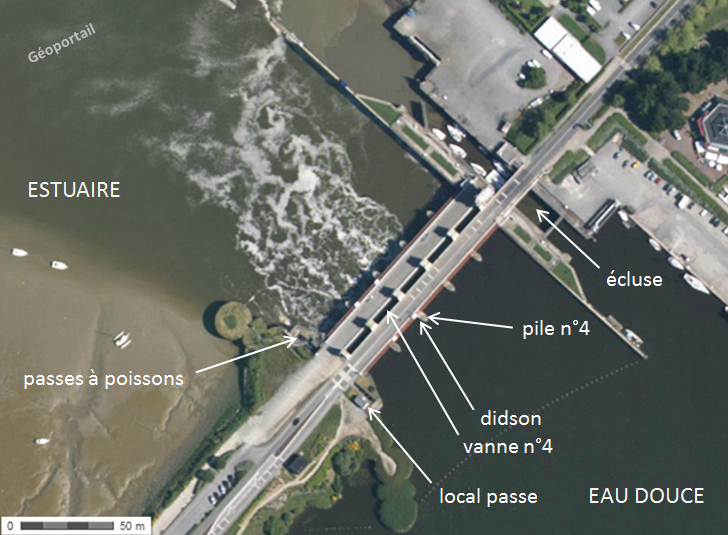
\includegraphics[width=0.5\textwidth]{vueaeriennebarrage.png}
\caption[Vue aérienne du barrage d'Arzal]{Vue aérienne du barrage d'Arzal,
montrant en rive droite l'écluse et le pertuis des vannes.}
\label{vueaeriennebarrage}
\end{figure}

Le sonar multifaisceaux est positionné 15 m en amont de la
vanne 4 (Figure \ref{arzal_aval}), dans l'échancrure de batardage de
la vanne.  La structure porteuse de l'appareil est une poutre HEB 240 de 12m, sa fixation permet de maintenir le didson à l'abri des corps
dérivants (Figure \ref{positionnementdidson}).

\begin{figure}[htbp]
\centering
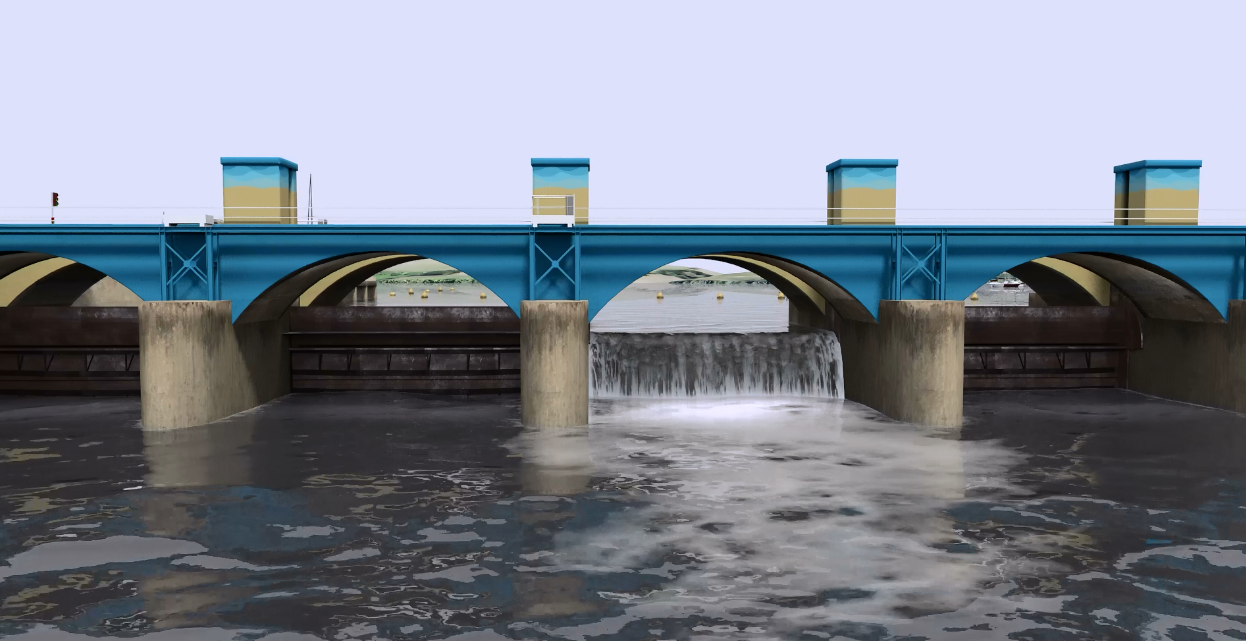
\includegraphics[width=0.5\textwidth]{arzal_aval}
\caption[Vue aval du volet]{Vue montrant un écoulement sur le volet 4 à
partir de l'aval du barrage.}
\label{arzal_aval}
\end{figure}


\begin{figure}[hbp]
\centering
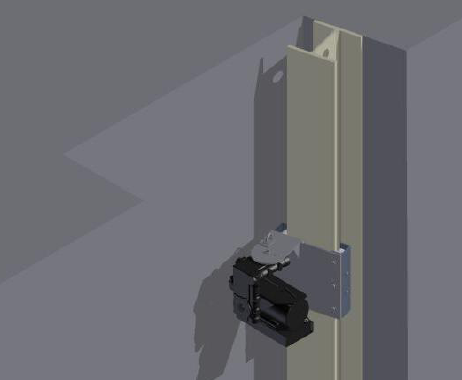
\includegraphics[width=0.5\textwidth]{positionnementdidson.png}
\caption[Positionnement du didson]{Positionnement du didson dans l'échancrure
de batardage de la vanne. Le didson est placé à l'abri des corps dérivants.}
\label{positionnementdidson}
\end{figure}








\subsection{Description du matériel}

Le système d'enregistrement est composé d'un sonar multifaisceaux (didson de
Soundmetrics) équipé par un rotateur (Soundmetrics, X2) permettant de guider le
didson dans un positionnement vertical et latéral (Figure
\ref{didson2017}). Le chariot du didson permet de le positionner à différentes
profondeurs dans la colonne d'eau (Figure
\ref{chariot}). Les images sont traitées à l'aide du logiciel de dépouillement
didson V5.27.48 de la société Soundmetrics. 



\begin{figure}[htbp]
\centering
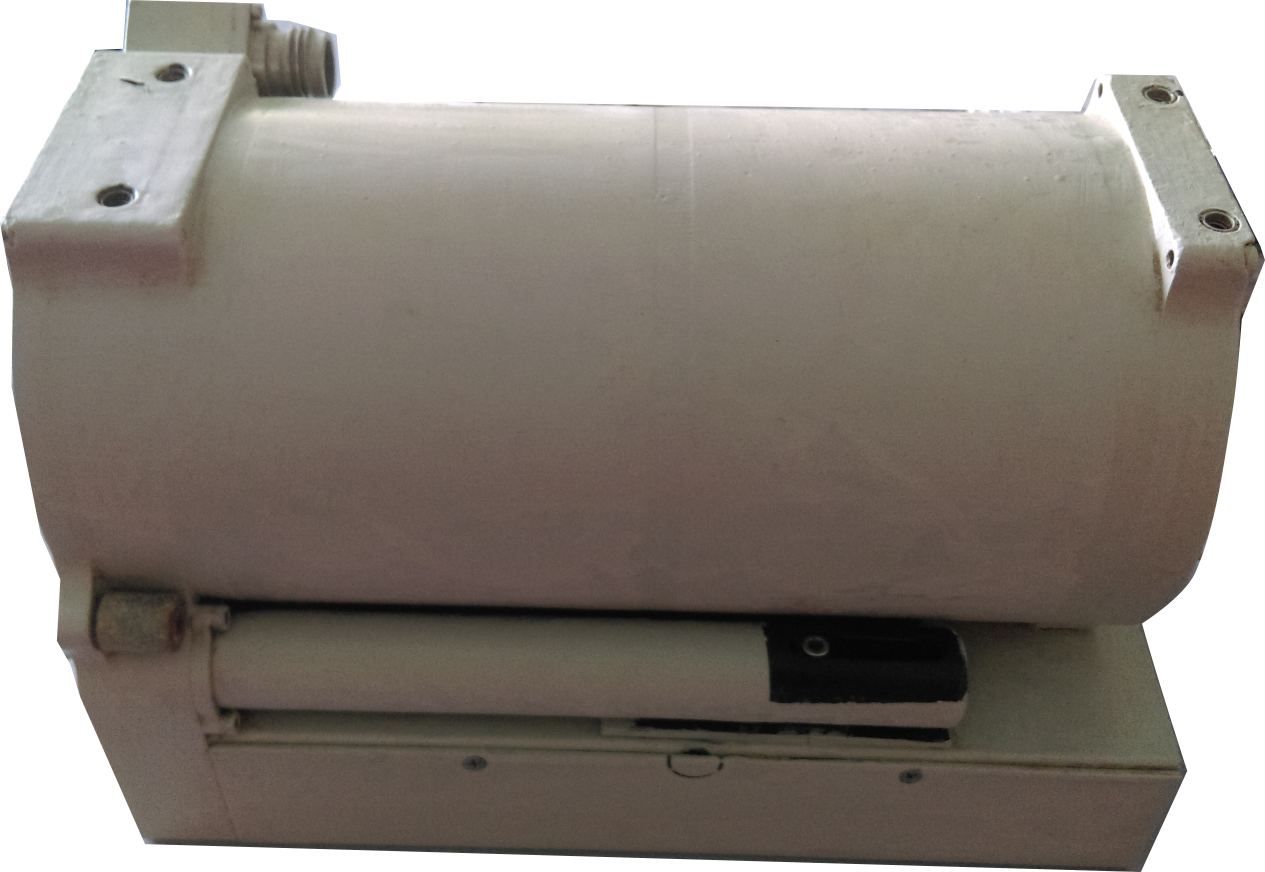
\includegraphics[width=0.3\textwidth]{didson.png}
\caption[Le didson en 2017]{Le didson en 2017.
}
\label{didson2017}
\end{figure}


\begin{figure}[htbp]
\centering
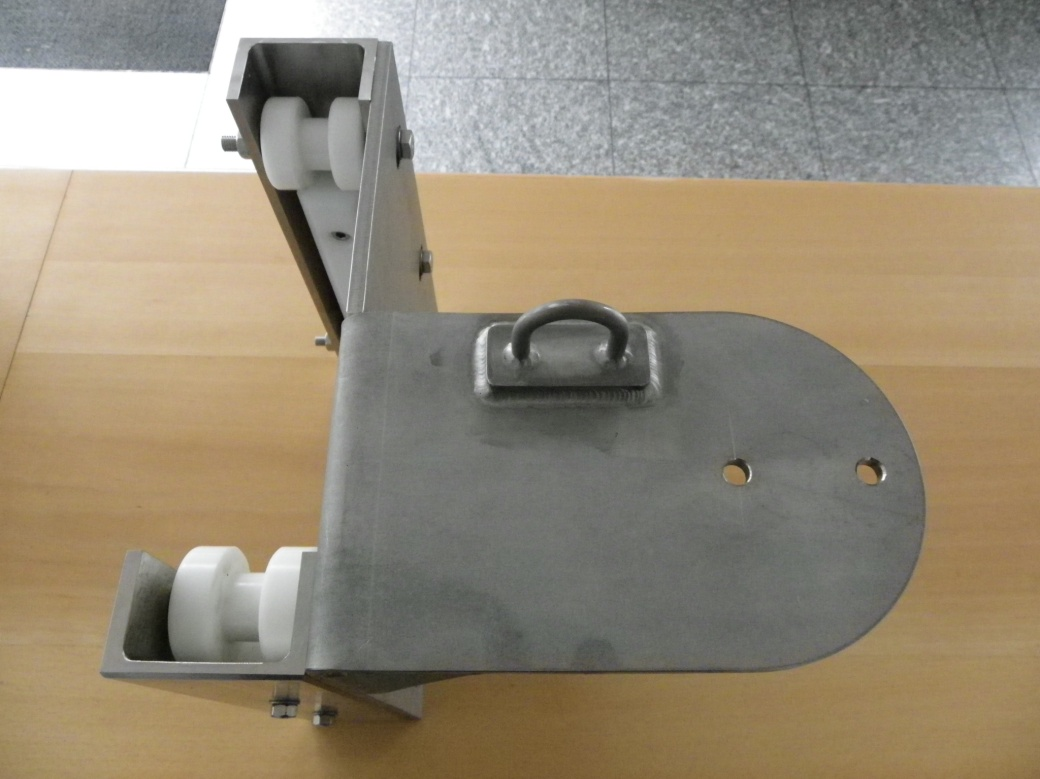
\includegraphics[width=0.3\textwidth]{chariot}
\caption[Chariot du didson]{Chariot du didson.}
\label{chariot}
\end{figure}

\subsection{Automatisation de la position verticale du didson}

La position verticale du didson est automatisée par un treuil. 
Le treuil est relié à l'automate du barrage par une liaison
ethernet et le pilotage des positionnements du didson se fait par une
interface graphique (Figures \ref{automate2} et \ref{ihm}).
Un système de gestion
des câbles permet le déplacement vertical du didson à l'aide un chariot (Figure
\ref{automate3}).

%------------------------------------------
\begin{figure}[htbp]
\centering
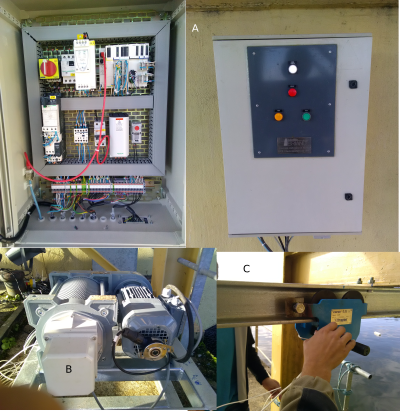
\includegraphics[width=0.5\textwidth]{automate2.png}
\caption[automatisation]{A Armoire électrique de commande du treuil,
déportée sur la pile, B treuil avec codeur incrémental, C chariot de levage et
de positionnement du didson (pour la sécurité). }
\label{automate2}
\end{figure}
%------------------------------------------
%------------------------------------------
\begin{figure}[htbp]
\centering
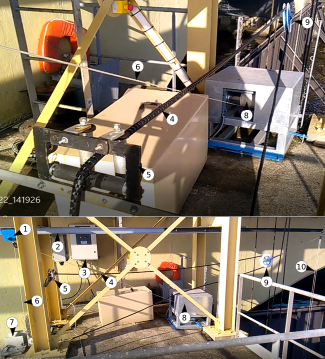
\includegraphics[width=0.5\textwidth]{automate3.png}
\caption[automatisation]{Automatisation de la position verticale du didson. 1
chariot sur poutre HEB, 2 rail, 3 coffret électrique comprenant les éléments de
contrôle de l'automate, 4 câble du didson (alimentation et signal) renforcé par une gaine, 5 guide
câble, 6 câble de traction du didson, 7 poutre HEB du chariot de didson
(plongeant en amont de la vanne), 8 treuil et chaise de protection, 9 poulie, 10 contrepoids assurant la
tension du câble. }
\label{automate3}
\end{figure}
%------------------------------------------
%------------------------------------------
\begin{figure}[htbp]
\centering
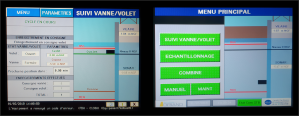
\includegraphics[width=0.5\textwidth]{ihm2.png}
\caption[automatisation]{Ecrans de contrôle et de programmation de la position
du didson}
\label{ihm}
\end{figure}
%------------------------------------------
\subsection{Suivi des migrations}

Lors de l'hiver 2012--2013, le didson avait été placé dans trois types de
positions. En position haute lorsque les écoulements étaient en
surface (Figure \ref{didsonsurface}). Lorsque l'écoulement s'effectuait
par le fond, en période de plus fort débit, il a été placé en position basse, à
80 cm du fond. Il a alors été programmé afin d'échantillonner alternativement
une zone où une partie de l'écho se reflétait sur le fond, et une zone en pleine
eau.\\

En 2013--2014, la stratégie d'échantillonnage a été revue : l'analyse des
données 2012--2013 montre que l'écho sur le fond a pu générer une perte
d'efficacité du didson dans la zone d'écho. L'enregistrement près du fond a continué à être
effectué à -6.92 m (80 cm du fond) mais les angles du didson ont été réglés à 4
et 6 ° pour que la zone d'acquisition reste en pleine eau. En surface,
l'acquisition a été faite à angle constant \ang{-7} afin que la
zone d'acquisition du didson reste sous la surface, pour éviter que les reflets à la surface de l'eau ne gênent la lecture (Figure
\ref{echo}).
Des essais ont également été effectués en surface, et au fond, en alternant
les directions du didson entre un angle élevé et une position droite,
pour tenter de collecter des informations sur 
la position verticale des anguilles en fonction
des ouvertures de la vanne.  \\

En 2014--2015, la gestion du positionnement du didson a été fortement dépendante
de la gestion de crise du barrage du fait des avaries répétées des vannes. Le
rotateur a été cassé lors de la principale crue, alors que la majeure partie du
débit a été évacuée sur la vanne 4.

En 2015--2016, le rotateur n'a été remplacé qu'au 4 janvier. Le didson a
fonctionné avec un angle constant pour le début de la saison. Il a été placé
alternativement en surface et au fond en fonction des débits du barrage. 
Du 4 janvier au 26 avril, la saison a été constituée d'une
succession de pics de crue d'ampleur moyenne, pendant lesquels le didson
a enregistré au fond. 

En 2016--2017, le didson a été bien positionné pour enregistrer les deux
premiers pics de crue. À partir du 13/02, le signal a été détérioré par une
attaque de corrosion. Jusqu'au 17/03, malgré plusieurs essais de remise en
fonctionnement, il n'y a pas vraiment de suivi. En fin de saison, le didson a
été placé en volet puis en vanne mais les effectifs observés sont restés
faibles.

En 2017--2018, un problème de déformation du concentrateur de faisceau (slit) a dégradé
la qualité des images à partir de fin janvier.

En 2018--2019, l'essentiel de la saison est couvert par le mode "suivi
vanne volet" qui permet de positionner correctement le didson en cours de
nuit lorsque la gestion du barrage alterne entre vannes en volets. 

En 2019--2020, la saison s'effectue avec un suivi principalement en vanne dès
le début de la saison. Le suivi a été arrêté le 19/02 après que le câble ait
été entaillé par un objet dérivant qui a mis fin au suivi (Figure
\ref{fig_effectif}). Cette situation intervient cependant après plusieurs pics
de crue et il est probable que l'essentiel de la migration ait eu lieu.

En 2020--2021 plusieurs problemes techniques ont lieu entre octobre et décembre, 
plantages liés à l'humidité, arrêts électriques à répétition sur l'ouvrage,
plantage de la mémoire vive du PC d'acquisition, problème de codeur et de fin de course sur le
volet, difficultés à mettre en service l'automatisme de suivi vanne volet...
Le didson fonctionne globalement plutôt bien sur le reste de la saison, qui
présente deux pics de crues importants en janvier et février avec des débits de
l'ordre de 700 $m^3.s^{-1}$. Le didson est enlevé de l'eau lors du deuxième pic
de crue le 03/02. 

En 2021--2022, en tout début de saison, il y a des difficultés à utiliser
l'automate du treuil du fait d'un problème de communication entre l'armoire
électrique de la pile et l'automate. Ces problèmes n'ont pas d'incidence car
l'appareil reste en surface. Par la suite l'utilisation de
l'automate permettra d'alterner les positions vanne et volet. 
Les problèmes d'acquisition sont liés à des problèmes électriques du
barrage et sont en général de faible durée (Figure \ref{fig_effectif_pb}).
Un seul pic de crue est observé en janvier avec des débits de l'ordre de 300
$m^3.s^{-1}$

En 2022--2023, il y a eu de nombreux plantages intempestifs du didson au cours de la saison.
La majorité de ces derniers sont liés à un problème d'accès au disque dur. 
Le rotateur commence également à montrer des signes d'usures.
La première crue à débutée le 20 décembre avec des débits de l'ordre de 
380 $m^3.s^{-1}$. Plus une diminution suivie d'une deuxième crue à partir 
du 31 décembre de l'ordre de 350 $m^3.s^{-1}$. 
Ces crues ont été suivies d'une période calme du 6 février au 9 mars, puis un
enchainement de 5 pics de crues jusqu'à la fin de la saison (en fin avril) 
avec des débits de l'ordre de 180 à 270 $m^3.s^{-1}$.

%------------------------------------------
\begin{figure}[htbp]
\centering
\includegraphics[width=0.5\textwidth]{didsonA}
\caption[schéma didson -7° 5-15m]{Schéma montrant la position du didson et
la fenêtre d'échantillonnage couverte par l'appareil lorsque celui-ci est placé
1 m sous la surface (-7°) pour détecter les anguilles migrant sur le volet.
Les polygones de couleur représentent les différentes sections
d'échantillonnage en fonction de la distance.}
\label{didsonsurface}
\end{figure}

\begin{figure}[htbp]
\centering
\includegraphics[width=0.5\textwidth]{didsonD1}
\caption[schéma didson 0° 5-15m]{Fond 0° 5-15m, didson placé à 5.5 m de
profondeur lorsqu'il alterne entre des positions au fond et en surface à l 'aide
du positionnement géré par l'automate. Le didson échantillonne 
\num[round-mode=places,round-precision=1]{14.8}\%
de la fenêtre de passage supposée. 
}
\label{didsonD1}
\end{figure}
\begin{figure}[htbp]
\centering
\includegraphics[width=0.5\textwidth]{didsonD2}
\caption[schéma didson -7° 5-15m]{Fond -7° 5-15m, didson placé à 4.5 m de
profondeur avec un angle de -7°. Par rapport à la position en
Figure \ref{didsonD1} le didson est remonté. L'angle de -7° permet d'éviter les
échos sur la surface lorsque le didson est remonté en position haute par l'automate. Le didson
échantillonne
\num[round-mode=places,round-precision=1]{14.6}\%
de la fenêtre de passage supposée.
}
\label{didsonD2}
\end{figure}

 
\subsection{Mesure des conditions environnementales}

Les paramètres décrivant le fonctionnement du barrage sont enregistrés toutes
les dix minutes dans la base de données SIVA \footnote{SIVA=Système
d'Information de la Vilaine et de ses Affluents}. Il s'agit :
\begin{enumerate}
\item Des niveaux d'ouverture des 5 vannes. 
\item De la position des volets, 5 clapets flottants par lesquels sont évacués
les débits du barrage lorsque le débit est suffisamment faible (entre 10 et 50 $m3^.s^-1$).
\item Des débits transitant par la
passe à poissons. 
\item Des débits des siphons \footnote{Les siphons sont des tuyaux dont le
fonctionnement gravitaire permet d'évacuer les lentilles d'eau salée
s'accumulant en profondeur en amont du barrage, du fait du fonctionnement
estival de l'écluse. Les siphons débouchent près de l'entrée de la passe en
rive gauche de l'ouvrage.}. 
\item Du débit de la Vilaine, calculé au niveau
du pont de Cran, 30 kilomètres en amont du barrage d'Arzal.
\item Des températures d'eau enregistrées au niveau de sondes en amont
et en aval du barrage.
\item Des niveaux d'eau enregistrés en amont et en aval du barrage sur plusieurs
sondes.
\end{enumerate}
Les données ont été collectées à partir de la base de données 
 et compilées par
séquences de 30 minutes dans un format compatible avec celui du didson.

D'autres données, au format journalier, comme les horaires de levers et couchers
du soleil, ont été ajoutées à cette base. Les durées de pénombre civile correspondant à une position
du soleil entre 0° et -6° ont été estimées à partir d'une durée de 24 minutes avant le lever 
et après le coucher du soleil.
\subsection{Calcul des débits}
Les débits ont été re-calculés au droit du barrage d'Arzal car les formules de
débit étaient fausses, particulièrement en période de forts débits, où
les formules en écoulement libres conduisaient à sous-estimer les
débits. Les formules ont été recalculées à partir des débits de la station du
pont de Cran 30 km en amont du barrage. Les nouveaux débits sont donnés pour les volets 
et pour les vannes avec la prise en compte de plusieurs formules en fonction des
conditions d'écoulement (orifice dénoyé, orifice noyé, écoulement libre)
\citep{briand_note_2015}. L'ensemble des fonctions de calcul de débit sont
maintenant rassemblées au sein du package
\href{https://github.com/Eaux-et-Vilaine/SIVA}{SIVA} (Figure \ref{debits_ajustes}).

\begin{figure}[htbp]
\centering
\includegraphics[width=0.5\textwidth]{2023/debits_ajustes2023}
\caption[Débits recalculés 2023]{Débits recalculés en 2023.
Comparaison des débits mesurés au niveau de la station de Rieux (Pont de Cran - station
hydrométrique), des débits calculés par l'automate du barrage d'Arzal et des
débits recalculés par la méthode de \citet{briand_note_2015}.}
\label{debits_ajustes}
\end{figure}

L'analyse des données de débit des volets montre un fonctionnement régulier en
2022-2023 (Figure \ref{debitvoletjour}).

\begin{figure}[htbp]
\centering
\includegraphics[width=0.5\textwidth]{2023/debitvolet2023}
\caption[Débits volet 2023]{Débits recalculés sur chaque volet après correction
des dérives du codeur \citep{briand_note_2015}.}
\label{debitvoletjour}
\end{figure}

Les débits ont été recalculés pour chacun des pertuis de vanne
(Figure \ref{debits_inst2023}).

\begin{figure}[htbp]
\centering
\includegraphics[width=0.5\textwidth]{2023/debits_inst2023}
\caption[Débits sur chaque pertuis de vanne pour l'hiver 2022--2023]{Débits de
chacun des pertuis de vanne pour l'hiver 2022--2023 en
fonction des différents types d'écoulements calculés
sur chaque vanne \citep{briand_note_2015}.}
\label{debits_inst2023}
\end{figure}

\subsection{Dépouillement des fichiers}\label{par_depouillement}

Les fichiers sont recueillis au niveau du local de la passe à intervalles réguliers et rapatriés 
au siège de l'EPTB Vilaine. Ils sont ensuite traités par le logiciel
soundmetrics pour réduire le temps de dépouillement.
Le traitement (CSOT) retire les éléments stables de l'image (échos constants) et ne retient que des
poissons, des objets, voire rien en période de fort débit et forte turbidité. Ce
processus permet de réduire la taille des fichiers et de limiter le temps de dépouillement, mais il dépend aussi des conditions. Le passage d'un banc de mulets,
par exemple, pourra conduire à garder l'ensemble du fichier. 
Les seuils de traitement appliqués sont identiques aux années précédentes, 2.8 dB en volet et 2.5 dB en vanne.
Les fichiers qui contenaient des anguilles douteuses (notées 1 sur une échelle de 1 à 5) ont été relus par les deux lecteurs pour validation. 
La présence de mulets en dévalaison ou de nombreux alevins est notée sur une échelle de 0 à 5, 
depuis le niveau zéro (pas d'alevins ou de mulets) à 5 (gêne maximale).

Trois type de nage sont notés : 
\begin{itemize}
\item \emph{Running} l'anguille dévale normalement,
\item \emph{Backsliding} l'anguille dévale avec la tête orientée vers l'amont,
\item \emph{Hanging} l'anguille a un comportement de nage à contre courant et au
final il est difficile de savoir si elle est passée ou pas, ce type de
comportement se produit en général à l'ouverture des vannes.
\end{itemize}
Par rapport à la lecture du didson, les opérateurs renseignent également
l'entrée et la sortie des anguilles du champ. La zone d'écho du sonar se
présente comme un cône (Figure \ref{fig_anguilles}). Cette image rassemble en
deux dimensions les échos enregistrés à plusieurs hauteurs, il n'est donc pas
possible de connaître le positionnement vertical de l'anguille dans le cône du
faisceau (Figure \ref{didsonsurface}). Plusieurs types d'enregistrement sont
donc répertoriés :
\begin{itemize}
\item \emph{<-->} l'anguille traverse l'ensemble du champ horizontal prospecté
par le didson (elle traverse le faisceau d'un bord à l'autre (Figure
\ref{fig_anguilles})),
\item \emph{In} l'anguille entre dans le champ, soit par-dessus, soit par
dessous, soit latéralement (dans ce cas elle entre généralement en début de
champ de détection, c'est à dire qu'elle était entre la pile et la zone de
prospection); pour l'observateur elle apparaît donc en cours de trajectoire au milieu du champ,
\item \emph{Out} l'anguille sort du champ,
\item \emph{InOut} l'anguille entre et ressort.
\end{itemize}

\subsection{Traitements}

\label{partraitement}
Les données sont récupérées depuis la base de données PostgreSQL à l'aide
d'outils RODBC et DBI
\citep{conway_RPostgreSQLInterfacePostgreSQL_2021, wickham_2022}.

Les suivis concernent quatre classes de tailles d'anguilles ($\tau$ formule \ref{eq_tau}) dont les probabilités de détection par le didson ne sont pas
équivalentes en fonction des distances ($\delta$, formule \ref{eq_delta}, Figures
\ref{didsonsurface} \ref{didsonD1}).
La fenêtre de détection est découpée en cinq quadrilatères situés à des
distances croissantes $\delta$ (formule \ref{eq_delta}).
Les résultats ont été regroupés en fonction de deux positions du didson ($k$, formule
\ref{eq_k}). Les suivis sont ramenés à la durée d'un fichier de suivi, c'est à dire $t$=30 minutes.
Les données sont séparées par saison de suivi de 2012-2013 à 2022-2023.
%%%%%%%%%%%%%%%%%%%%%%%%%%%%%%%%%%%%%%%%%%%%%%%%%%%%%%%%%%%
\begin{equation}
  \label{eq_tau}
  \text{Tailles d'anguilles}~(\tau)=
  \begin{cases}
      <45cm~\text{mâles}\\
      45-60cm~\text{petites femelles}\\
      60-80cm~\text{femelles}\\
      >80cm~\text{grandes femelles}
  \end{cases}
\end{equation}
\begin{equation}
  \label{eq_delta}
  \text{Distance}~(\delta)=
  \begin{cases}
      (2,5m[\\
      (5,7m[\\
      (7,9m[\\
      (9,11m[\\
      (11,13m[\\
      (13,15m[      
  \end{cases}
\end{equation}
Les positions du didson au cours des différentes années de suivi peuvent se
résumer à 4 configurations,  sl correspond à un appareil penché pour essayer
d'évaluer le positionnement vertical des anguilles dans la lame d'eau.
\begin{equation}
  \label{eq_k}
  \text{Position}~(k)=
  \begin{cases}
      f_{5}~\text{fond, 5-15m}\\
      f_{3}~\text{fond, 3-12m}\\      
      s~\text{surface, 5-15m}\\
      sl~\text{fond et surface, 3-12m}\\
  \end{cases}
 \end{equation}
%%%%%%%%%%%%%%%%%%%%%%%%%%%%%%%%%%%%%%%%%%%%%%%%%%%%%%%%%%%
L'objectif des traitements est
d'extrapoler le nombre d'anguilles observées au niveau du sonar
$N_{4o}(t,\tau,\delta)$, à l'ensemble de la vanne 4, $N_4(t,\tau)$, puis à 
l'ensemble du fleuve Vilaine $N(t,\tau)$. 

\subsubsection{Efficacité de la détection}\label{par_traitement_efficacite}

Le nombre observé par les opérateurs du didson pour chaque classe de
taille, correspond au nombre d'anguilles
migrant multiplié par l'efficacité du didson $E_k(t,\delta,\tau,t)$, calculée pour
chaque classe de taille $\tau$ , chaque classe de distance $\delta$ et pour les
différentes positions du didson $k$ (Formule \ref{eq_efficacite}).
%%%%%%%%%%%%%%%%%%%%%%%%%%%%%%%%%%%%%%%%%%%%%%%%%%%%%%%%%%%
\begin{equation}
\label{eq_efficacite}
N'_{o4}(t,\tau,\delta,k)= N_{o4}(t,\tau,\delta,k) \times E_k(t,\delta,\tau)\\
\end{equation} 
%%%%%%%%%%%%%%%%%%%%%%%%%%%%%%%%%%%%%%%%%%%%%%%%%%%%%%%%%%%
Le nombre de détections disponibles pour le didson est trop faible
pour permettre de tester une variation temporelle de l'efficacité du didson et
la somme des effectifs observés sur l'ensemble de chaque saison et pour chaque
position du didson sert de base au calcul.
$$N_{o4}(\tau,\delta,k)=\sum_t N_{o4}(t,\tau,\delta,k,t)$$
Si l'efficacité était de 100\%, le nombre d'anguilles détectées devrait
augmenter régulièrement avec la distance au didson en proportion de
l'augmentation de la surface couverte par le faisceau $S(k)$ (Figure \ref{didsonsurface}). 

%%%%%%%%%%%%%%%%%%%%%%%%%%%%%%%%%%%%%%%%%%%%%%%%%%%%%%%%%%%
\begin{equation}
\label{eq_efficacite2}
\begin{aligned}
&N_{o4}(\tau,\delta+1,k)=\\
&N_{o4}(\tau,\delta,k) \times \frac{S(\delta+1,k)}{S(\delta,k)}
\end{aligned}
\end{equation} 
%%%%%%%%%%%%%%%%%%%%%%%%%%%%%%%%%%%%%%%%%%%%%%%%%%%%%%%%%%%
Les surfaces des polygones sont calculées par
l'intersection de droites \citep{murdoch_GpclibGeneralPolygon_2020} (Figures
\ref{didsonsurface}).
D'une classe de taille à la suivante, les nombres
observés devraient théoriquement augmenter en cohérence avec les rapports de
surface. Ainsi, cette augmentation devrait être
linéaire, sauf lorsque le faisceau heurte le fond, car alors une partie de la
zone de détection est perdue (cas pour les premières années de suivi).

En effet, d'après \ref{eq_efficacite} et \ref{eq_efficacite2}, on a (formule
\ref{eq_efficacite3}) :
%%%%%%%%%%%%%%%%%%%%%%%%%%%%%%%%%%%%%%%%%%%%%%%%%%%%%%%%%%%
\begin{equation}
\label{eq_efficacite3}
\begin{aligned}
& E(\delta+1,\tau,k)=\\
& E(\delta,\tau,k)\times\frac{S(\delta+1,k)}{S(\delta,k)}\times\frac{N'_{o4}(\tau,\delta,k)}{N'_{o4}(\tau,\delta+1,k)}\\
\end{aligned}
\end{equation} 
%%%%%%%%%%%%%%%%%%%%%%%%%%%%%%%%%%%%%%%%%%%%%%%%%%%%%%%%%%%

En pratique, les effectifs n'augmentent pas avec la surface de détection, et la
diminution dépend de la classe de taille. Les rapports des effectifs corrigés de
la taille du faisceau servent de base au calcul de l'efficacité (hypothèse 1, 
Figure \ref{fig_diag_efficacite})

En prenant comme référence E=1 pour
les classes de distance où les détections sont maximales, on pourrait calculer
l'efficacité pour chacune des classes de taille en fonction de la distance de
détection. Cette approche a été utilisée jusqu'en 2019-2020.
Le problème est que pour chaque classe de taille, la classe de
distance pour laquelle il y a le plus d'anguilles dans les effectifs corrigés se
voit attribuer la note de 1. Or un examen des qualités de détection montre clairement
un contraste entre les positions $k=$ volet ou vannes et en fonction
des classes de distance au didson et de la taille (Figure
\ref{qualite_distance}).
Les distances au didson sont déjà prises en compte dans le calcul des
efficacités, il reste donc à prendre en compte la diminution des efficacités en
fonction de la position et de la taille. L'idée est que la proportion
d'anguilles douteuses (et donc écartées des comptages) est proportionnelle
à la proportion d'anguilles de bonne qualité observée pour
les deux positions $k$, et pour les différentes classes de taille $\delta$ (hypothèse 3, 
Figure \ref{fig_diag_efficacite}).
A partir de 2019-2020, au lieu d'attribuer 1 comme maximum de classe, on
attribue la valeur $q$ qui est le rapport entre le pourcentage d'anguilles de bonne
qualité (4 ou 5) dans la classe de taille observée et la classe de référence :
$\tau=>80cm, k =surface$. En outre, les données sont analysées sur les détections de toutes les saisons (Figures
\ref{qualite_distance_volet_all}, \ref{qualite_distance_vanne_all}).

\begin{figure}[htbp]
       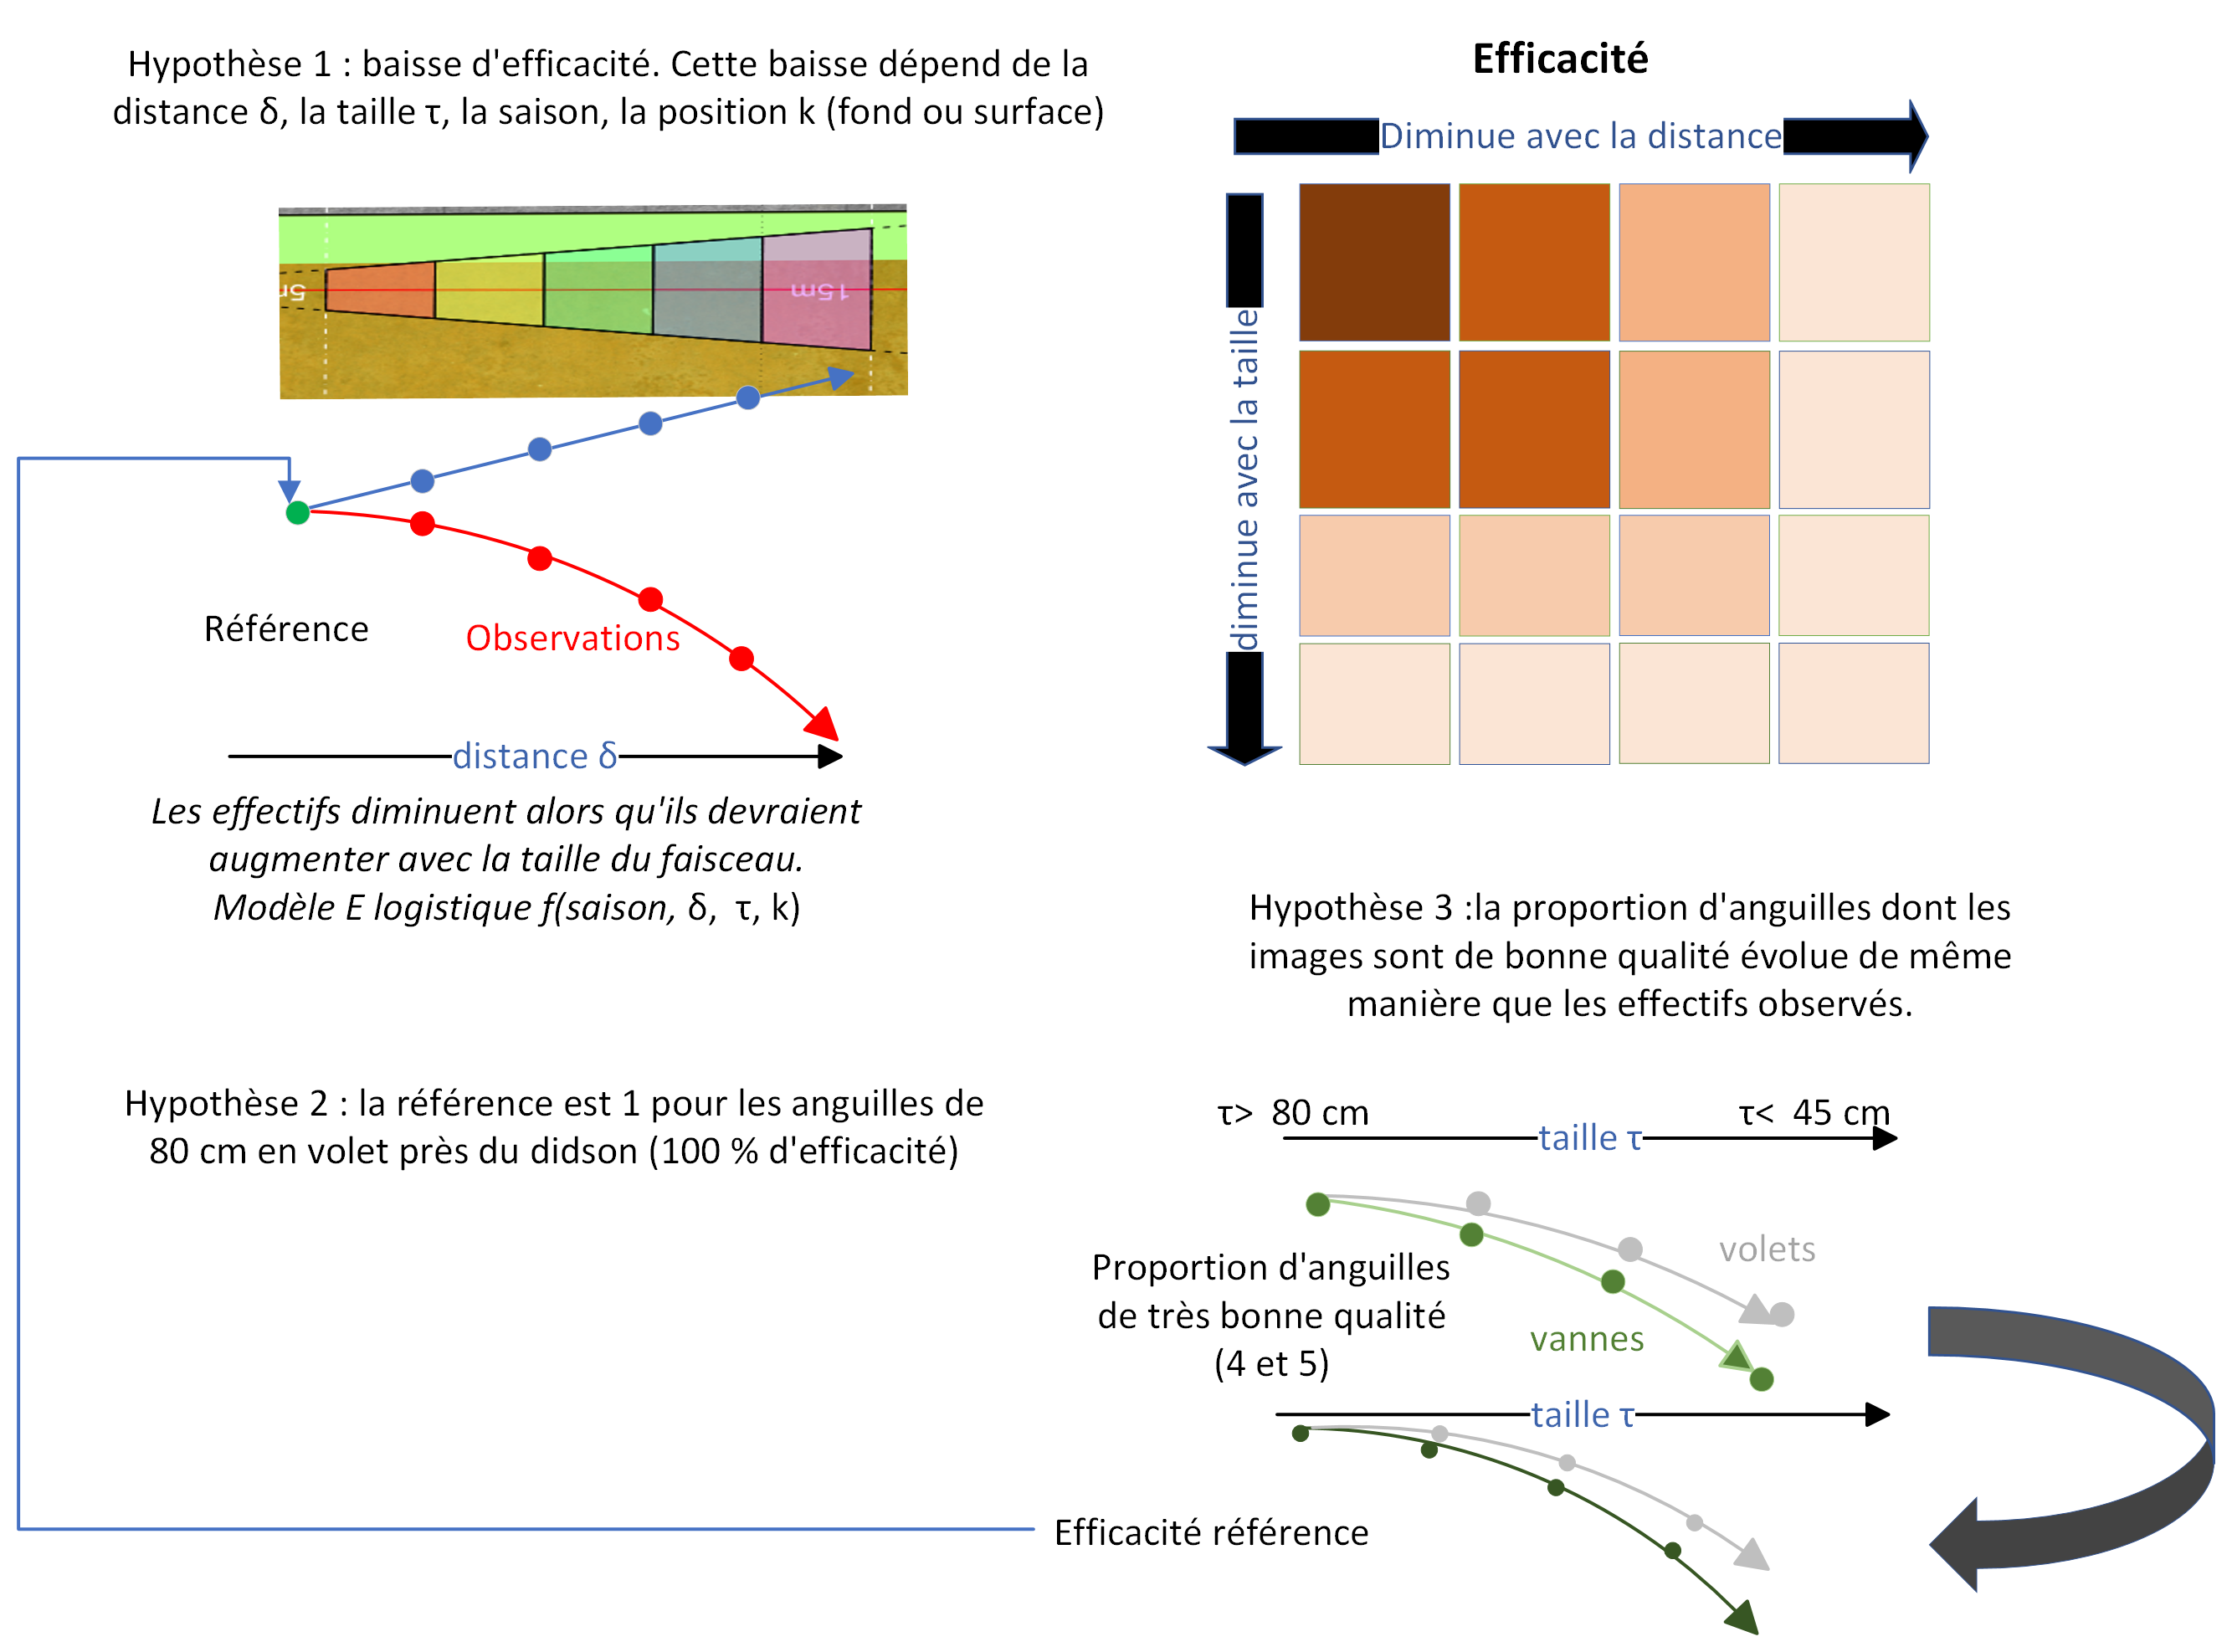
\includegraphics[width=0.5\textwidth]{visio_efficacite_didson.png}
        \caption[Diagramme efficacité.]{Diagramme schématique du calcul de
        l'efficacité.}
       \label{fig_diag_efficacite} 
\end{figure}

On fait l'hypothèse que pour la classe de distance la plus favorable et pour la
position volets, toutes les anguilles sont détectées (efficacité 1). Cette
hypothèse est probablement juste car il n'y a que des anguilles de bonne qualité (>2) 
pour les deux distances les plus proches du
didson dans la classe de taille >80cm.

Ces données sont ensuite utilisées pour calculer les efficacités moyennes par un modèle linéaire, pour lequel $b_0$, $b_1$,\dots,
$b_6$ sont les coefficients de la régression.
La distance, la position, la saison (avec une séparation pour les deux premières
saisons en fonction de la position de départ à 3 ou 5 m). Les interactions entre
la distance et la position $\delta:k$ et entre la taille et la position $\tau:k$ et avec la saison de suivi sont testées. 
 La prédiction du modèle peut conduire à des efficacités supérieures à 1, qui
 sont alors ramenées à 1 (formule \ref{eq_efficacite31}).
\begin{equation}
\label{eq_efficacite31}
\begin{aligned}
&\widehat{E(\delta,\tau,k)} = \\
min(1,&\\
&b_0+b_1\tau+b_2\delta+b_3 k+\\
&b_4\delta:k+b_5\tau:k+b_6 saison\\
)&
\end{aligned}
\end{equation} 
L'efficacité pour chaque position du didson k $\bar{E_k}$
correspond à l'efficacité moyenne pondérée, calculée comme suit :
\begin{equation}
\label{eq_efficacite32}
\bar{E_k}=\frac{\sum_{\tau \delta}N'_{o4}(\tau,\delta,k) }{\sum_{\tau \delta}N_{o4}(\tau,\delta,k)}
\end{equation} 
Le rotateur n'a pas été utilisé en 2018--2019. Les autres années, le calcul
des effectifs à chaque pas de temps était finalement pondéré d'un facteur lié au
temps d'enregistrement réduit par le fonctionnement du rotateur lorsqu'il se
repositionnait. Les enregistrements de chaque heure H étaient alors sur les
périodes $\text{H:00:00}$ $\Rightarrow$ $\text{H:29:00}$ et $\text{H:30:00}$ $\Rightarrow$ $\text{H:59:00}$. 
Sur les périodes correspondant à un échantillonnage en alternance, les effectifs
étaient donc amputés d'un facteur $\rho(k)$. Pour l'ensemble de la saison, en
l'absence de fonctionnement du rotateur, on a $\rho(k)$= 1.

\begin{equation}
\label{eq_efficacite4}
\begin{aligned}
\bar{E(k)}=&\bar{E(\delta,\tau,k)}\\
N'_{o4}(t,k)=& N_{o4}(t,k) \times \bar{E(k)} \times \rho(k)
\end{aligned}
\end{equation} 

\begin{figure}[htbp]
        \centering
        \begin{subfigure}{0.2\textwidth}
                \centering
                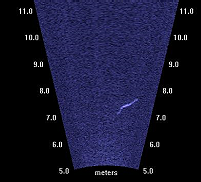
\includegraphics{anguille_114}
                \caption{Anguille de 114 cm.}
       \end{subfigure}%         
       \quad
        \begin{subfigure}{0.2\textwidth}
                \centering
                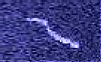
\includegraphics{anguille_detail}
                \caption{Détail anguille 83 cm.}
       \end{subfigure}%         
       \quad
      \begin{subfigure}{0.4\textwidth}
                \centering
                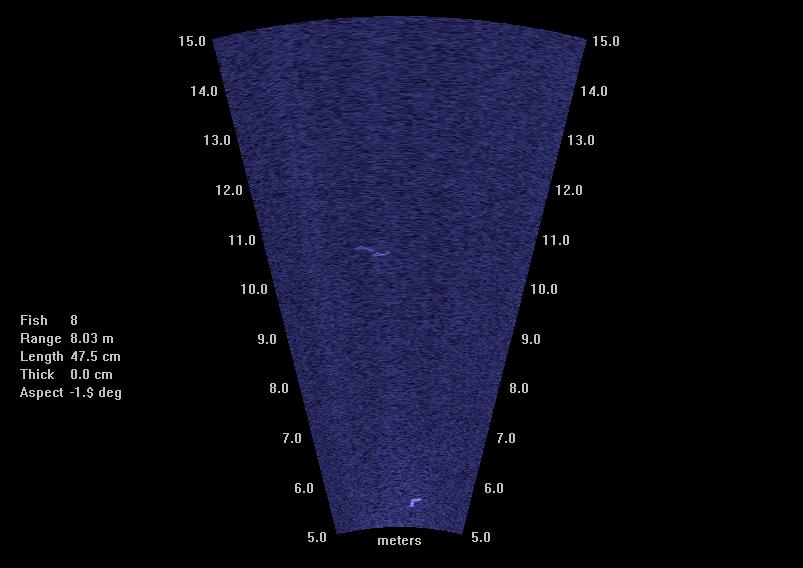
\includegraphics{anguilles}
                \caption{Deux anguilles}
                \label{ang0}
        \end{subfigure}%    
        \caption[Anguilles.]{Anguilles en dévalaison filmées par le didson.}
       \label{fig_anguilles}
\end{figure}

\subsubsection{Migration sur l'ensemble de la vanne}



Lors des écoulements par le fond, en vanne, l'analyse de la répartition
verticale des anguilles a montré qu'il semblait y avoir une présence des
anguilles sur l'ensemble de la colonne d'eau \citep{briand_suivi_2015}.
Compte tenu de cette observation, il a été nécessaire d'étendre la
hauteur de migration qui lors de la première année n'avait été considérée que comme étant
de deux fois la hauteur d'ouverture de la vanne. Nous faisons l'hypothèse que
les anguilles migrent sur l'ensemble de la colonne d'eau à l'exception des deux mètres en surface ($\Lambda$=2). 

L'examen des comportements d'anguilles dans
le fond de la vanne, lorsque les écoulements s'effectuent en volet (par le
clapet de surface), montre que ces dernières ne sont pas affectées par les écoulements en surface. 

Au contraire, en surface, on observe bien un comportement de migration
verticale, avec une montée dans la colonne d'eau, qui se traduit par une
apparition et une disparition des anguilles du faisceau du didson et non une
traversée comme c'est plus souvent le cas lorsque les écoulements sont linéaires
au fond. En surface, les migrations sont donc extrapolées sur une zone
représentant $\lambda$=6 fois la charge sur le volet. Ainsi, pour toutes les
années de suivi, la même approche a été utilisée : le nombre passant au niveau
de la vanne correspond au nombre passant dans le cône de détection du didson $N_{o4}$, 
extrapolé à l'ensemble de la fenêtre de migration.

Le ratio des surfaces F dépend donc de la hauteur de la colonne d'eau  $D_t$ ou
de la charge sur le volet $C_t$ qui est calculée à chaque pas de temps (formules
\ref{eqmigvan1} et \ref{eqmigvan2}). 
\begin{equation}
\label{eqmigvan1}
 N_{o4}(t,k)=N_4(t,k)) \times F(t,k,\Lambda,\lambda)\\
\end{equation}
 
 \begin{equation}
\label{eqmigvan2}
 F(t,k,\Lambda,\lambda)=
 \begin{cases}
\frac{S(k)}{l (D_t-\Lambda)} \text{au fond}\\
\frac{S(k)}{l C_t \lambda} \text{en surface}
\end{cases}
 \end{equation}
 
\subsubsection{Migration sur l'ensemble du barrage}

Nous faisons l'hypothèse qu'il n'y a pas de trajet de migration préférentielle
au droit du barrage, c'est à dire que la répartition des anguilles entre les
différents pertuis se fait au \textit{prorata} du débit. 
%%%%%%%%%%%%%%%%%%%%%%%%%%%%%%%%%%%%%%%%%%%%%%%%%%%%%%%%%%% 
\begin{equation}
\label{eq_Ntotal}
N_4(t) = \frac{Q_4(t)} {Q(t)} \times N(t)\\
\end{equation}
%%%%%%%%%%%%%%%%%%%%%%%%%%%%%%%%%%%%%%%%%%%%%%%%%%%%%%%%%%%

\subsubsection{Migration jour/nuit}

Comme les anguilles migrent majoritairement de nuit, les dépouillements ont été
effectués sur les fichiers correspondant à la période nocturne. Pour la
migration diurne, le pourcentage d'anguilles migrant de jour $\mu$ a été calculé.
\begin{equation}
\label{eq_mu}
N = \frac{\sum_{t=nuit}N}{1-\mu}\\
\end{equation}

\subsubsection{Modélisation de la migration}
Nous avons reconstitué les
effectifs en migration lors des périodes sans suivi $N_d\otimes$ à partir des densités mesurées 
pour la même nuit dans un positionnement correct $N_d\odot$ et du volume d'eau
transitant par le barrage $V\odot$ (Equation \ref{mod}).
\begin{equation}
\label{mod}
N_d\otimes=\frac{\sum_{t,k} N(t,k)\odot*V\otimes}{V\odot}
\end{equation}
Pour les jours où aucun suivi n'a été effectué à cause de problèmes
techniques les effectifs $N_d\oplus$ ont été interpolés à partir de la tendance
des effectifs journaliers par un modèle gam basé sur la
tendance saisonnière et le débit.

\subsubsection{Calcul des biomasses}

Les biomasses en dévalaison ont été calculées à partir de la fréquence de taille
corrigée des anguilles à moins de 7 m de distance du didson. Les fréquences des
effectifs de chaque classe de taille de 5cm ont été calculées et multipliées par le poids moyen du centre de la
classe, tel que prédit par la relation taille/poids calée sur les données régionales
d'anguilles argentées (source OFB et EPTB-Vilaine).

%%%%%%%%%%%%%%%%%%%%%%%%%%%%%%%%%%%%%%%%%%%%%%%%%%%%%%%%%%%
%\newpage
\section{Résultats}
\subsection{Suivi}
\subsubsection{Fonctionnement du barrage}



Le barrage ne commence à ouvrir qu'en novembre à la date de la mise en place du
didson (Figures \ref{debitturbidite} et \ref{fonctionnementvanne}). Trois
grosses crues sont observées (débit supérieur à
\SI{300}{\cubic\metre\per\second}) entre mi-décembre et mi-janvier, puis mars
des pics successifs entre 100 et 200 \unit{\cubic\metre\per\second}.
Les
turbidités montent au-delà de 100 NTU au cours de la crue de
décembre-janvier (Figure \ref{debitturbidite}).

\begin{figure}[ht!]
  \centering
  \includegraphics[width=0.4\textwidth]{2023/debitturbidite.png}
  \caption[Débits, turbidité et problèmes de fonctionnement du
  sonar]{ Débit de la Vilaine 
  (m$^3$.s$^{-1}$ \textcolor{black}{\rule[0.5mm]{0.5cm}{0.3mm}}) et turbidité
  (NTU, \protect\dashedrule) pendant la période de migration. En
  \textcolor{turquoise_EV}{\rule[-0.5mm]{3mm}{2mm}} débits corrigés (moyennes journalières). En fond, problèmes de fonctionnement du sonar,
   en jaune \textcolor{jaune_EV}{\rule[-0.5mm]{3mm}{2mm}} erreurs ponctuelles
  d'acquisition, %en jaune, \textcolor{yellow}{\rule[-0.5mm]{3mm}{2mm}}
  % problèmes d'écriture,
  en orange, \textcolor{orange_EV}{\rule[-0.5mm]{3mm}{2mm}} problèmes
 de qualité (absents cette année), 
  voir aussi la figure
\ref{fig_horairespb} dans la discussion pour le détail des horaires.}
  \label{debitturbidite}
\end{figure}

\begin{figure}[ht!]
  \centering
  \includegraphics[width=0.4\textwidth]{2023/fonctionnementvanne.png}
  \caption[Fonctionnement du barrage]{Fonctionnement du barrage, ouverture de la
  vanne 4 et du volet 4 et débit de la Vilaine pendant la période de migration.
  Chaque point correspond à une valeur pendant 30 minutes. 
  }
  \label{fonctionnementvanne}
\end{figure}



\subsubsection{Dépouillement des fichiers}
Le dépouillement correspond à du temps de lecture de fichier (Figure
\ref{tps}), il ne comprend pas la maintenance des
données, l'inscription dans la base ou les vérifications. 
En prenant comme base un temps de dépouillement de 6 heures par jour, 5
jours par semaine, la durée totale de dépouillement n'est que de l'ordre de
\num{6} semaines et
\num{3} jours contre 
\num{3} semaines et
\num{4} jours et 
\num{5} semaines et
\num{3} jour pour les deux
saisons précédentes (Tableau \ref{tabletps}). 


\input{../table/2023/depouillement.tex}
Cette année les temps de dépouillement sont de 10-20 minutes alors qu'ils
pouvaient être de 30 minutes lors des pics de migration, la mesure des anguilles
restant chronophage (Figure \ref{tpspoint}).
\begin{figure}[htbp]
        \centering
        \begin{subfigure}{0.4\textwidth}
                \centering
                \includegraphics{2023/tpspoint}
                \caption[Temps de dépouillement par fichier de 30
                minutes]{Temps de dépouillement en 2022-2023.}
                \label{tpspoint}
       \end{subfigure}%         
       \quad
      \begin{subfigure}{0.4\textwidth}
                \centering
                \includegraphics{2023/tpsboxplot}
                \caption[Temps de dépouillement par fichier de 30
                minutes]{BoxPlot des temps de dépouillement en 2022-2023.}
                \label{tpsboxplot}
        \end{subfigure}%    
        \caption[Temps de dépouillement, distribution et boxplot]{Temps de
        dépouillement, distribution et boxplot.}
              \label{tps}
\end{figure}
Cette année comme les autres, les fichiers ont été vérifiés grâce à la double
inscription des dépouillements, à la fois dans un fichier excel, et après
traitement des fichiers textes comprenant les données poisson.


Deux facteurs principaux gênent la lecture des fichiers du didson, il s'agit de
la présence d'alevins et de la présence de mulets. Les présences gênantes
d'alevins et de mulets peuvent exister en début de saison en octobre et novembre, 
sans toutefois constituer un facteur limitant pour le comptage. Ils
disparaissent en hiver avant de réapparaitre en mars (Figures \ref{mulet},
\ref{mulet2}, \ref{al}).


\begin{figure}[htbp]
  \centering
  \includegraphics[width=0.4\textwidth]{2023/mulet}
  \caption[présence de mulets lors des comptages]{Histogramme montrant la
  présence de mulets (\textcolor{orange_EV}{\rule[0.5mm]{0.5cm}{0.5mm}}) et 
  d'alevins (\textcolor{turquoise_EV}{\rule[0.5mm]{0.5cm}{0.5mm}}) dans les
  comptages, les valeurs sont aggrégées sous forme de moyenne à partir de scores
  allant de 0 (pas de poissons) à 5 (poissons très gênants pour le comptage).}
  \label{mulet}
\end{figure}
\begin{figure}[htbp]
  \centering
  \includegraphics[width=0.4\textwidth]{2023/mulet2}
  \caption[présence de mulets lors des comptages]{Importance de la présence
  des mulets par mois et en fonction de l'heure.}
  \label{mulet2}
\end{figure}
\begin{figure}[htbp]
  \centering
  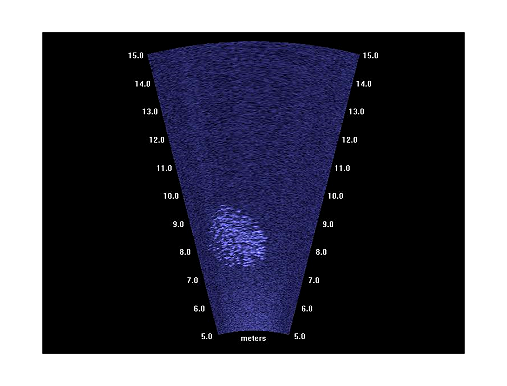
\includegraphics[width=0.4\textwidth]{alevin}
  \caption[Bancs d'alevins]{Banc d'alevins le 24 avril 2015.}
  \label{al}
\end{figure}
\begin{figure}[htbp]
  \centering
  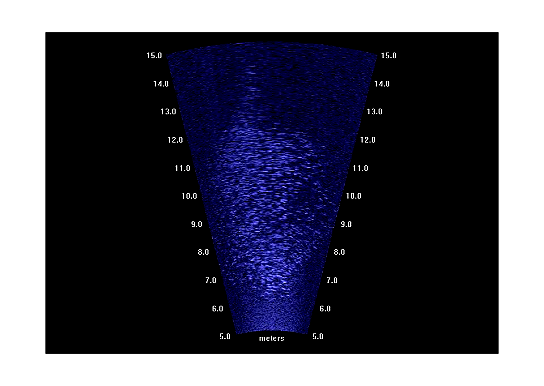
\includegraphics[width=0.4\textwidth]{alevin2}
  \caption[Banc d'alevins]{Banc d'alevins le 26 avril 2015.}
  \label{al2}
\end{figure}

Les mulets sont plus gênants que les alevins, avec une
lecture difficile dès que le score dépasse 2, ce qui n'est arrivé qu'en octobre
cette année. Les mulets ont toutefois une activité diurne et la gêne est
en général concentrée en début et fin de nuit.

%Il n'y a pas eu suffisamment de
%dépouillements de journées complètes en 2018--2019, et les valeurs diurnes /
%nocturnes de 2013--2014 ont été appliquées pour le calcul du coefficient $\mu$
%(Figure \ref{h_fonct}).


\begin{figure}[htbp]
  \centering
  \includegraphics[width=0.5\textwidth]{2023/horaires}
  \caption[Horaires de suivi]{Heures de début et de fin des fichiers
  dépouillés, et heures de lever et de coucher du soleil (en jaune). Les rectangles bleus
  à violet correspondent à des horaires de fichiers dépouillés, en noir pas de
  dépouillement, en orange début et fin des durées de pénombre civiles
  correspondant à une position du soleil à -6° en dessous de l'horizon.}
  \label{h_fonct}
  % heure de fonctionnement
\end{figure}

\subsubsection{Problèmes dans le suivi}
\label{parqualite}
\begin{figure}[htbp]
  \centering
  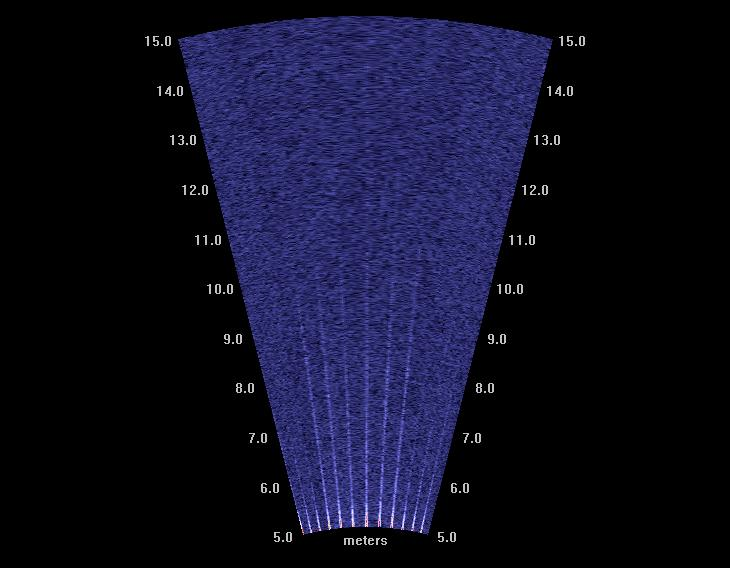
\includegraphics[width=0.4\textwidth]{flash}
  \caption[Interférence du didson]{Flash du didson}
  \label{flash}
\end{figure}
\begin{figure}[htbp]
  \centering
  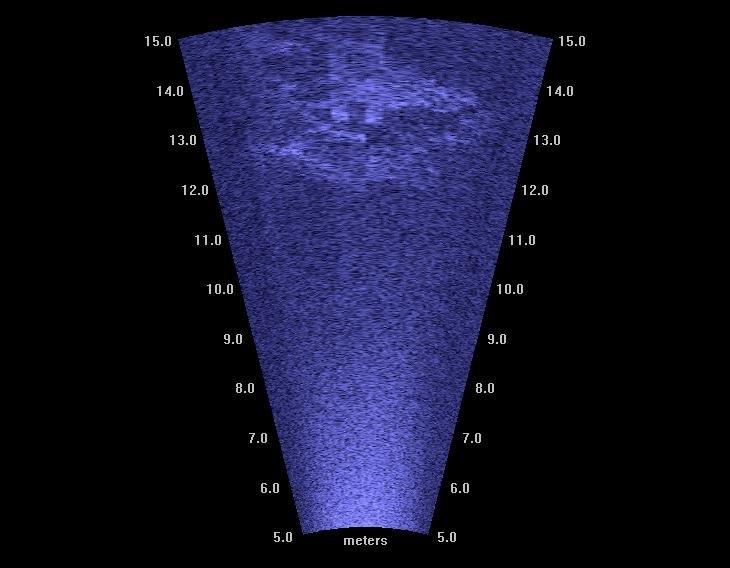
\includegraphics[width=0.4\textwidth]{echo_surface}
  \caption[Echo à la surface]{Echo du didson à la surface.}
  \label{echo}
\end{figure}

L'ensemble des problèmes techniques est résumé sur les Figures
\ref{debitturbidite}, \ref{fig_horairespb} pour le détail par 30 minutes, et \ref{fig_effectif_pb} pour le graphique saisonnier.

\input{../table/2023/tabfls.tex}
\input{../table/2023/tabflsall.tex}
\subsubsection{Positionnement du didson}


\begin{figure}[htbp]
        \centering
%        \begin{subfigure}{0.2\textwidth}
%                \centering
%                \includegraphics[trim=5mm 10mm 15mm 10mm,clip]{2021/position09}
%                \caption{Septembre}
%                \label{position09}
%       \end{subfigure}        
%       ~
        \begin{subfigure}{0.2\textwidth}
                \centering
                \includegraphics[trim=5mm 10mm 15mm 10mm,clip]{2023/position10}
                \caption{Octobre}
                \label{position10}
       \end{subfigure}        
       \quad
        \begin{subfigure}{0.2\textwidth}
                \centering
                \includegraphics[trim=5mm 10mm 15mm 10mm,clip]{2023/position11}
                \caption{Novembre}
                \label{position11}
       \end{subfigure}        
       ~
        \begin{subfigure}{0.2\textwidth}
                \centering
                \includegraphics[trim=5mm 10mm 15mm 10mm,clip]{2023/position12}
                \caption{Décembre}
                \label{position12}
       \end{subfigure}        
       \quad
        \begin{subfigure}{0.2\textwidth}
                \centering
                \includegraphics[trim=5mm 10mm 15mm 10mm,clip]{2023/position01}
                \caption{Janvier}
                \label{position01}
       \end{subfigure}        
       ~
        \begin{subfigure}{0.2\textwidth}
                \centering
                \includegraphics[trim=5mm 10mm 15mm 10mm,clip]{2023/position02}
                \caption{Février}
                \label{position02}
       \end{subfigure}        
       \quad
        \begin{subfigure}{0.2\textwidth}
                \centering
                \includegraphics[trim=5mm 10mm 15mm 10mm,clip]{2023/position03}
                \caption{Mars}
                \label{position03}
       \end{subfigure}        
        ~
        \begin{subfigure}{0.2\textwidth}
                \centering
                \includegraphics[trim=5mm 10mm 15mm 10mm,clip]{2023/position04}
                \caption{Avril}
                \label{position04}
       \end{subfigure}        
    \caption[Position du didson par rapport à la vanne 4]{Position du didson et de
    la vanne 4, taille des rectangles relative au nombre d'occurences d'un type
    de positionnement de vanne et d'un type de positionnement didson pour chaque mois.
    En lignes, positionnement du didson, 00 = pas de données, 0 = pas de
    lecture, s = surface (Figure \ref{didsonsurface}), f=fond (Figure \ref{didsonD1}).
    En colonnes, ouverture de la vanne, 0= pas d'ouverture, s=surface, f=fond,
    sf= surface et fond (l'ouverture change au cours des 30 minutes). 
    
    Couleurs :
    \textbf{\textcolor{orange_EV}{orange}} le didson n'enregistre
    pas pour des raisons techniques, \textbf{noir} vanne fermée, \textbf{\textcolor{Gray}{gris}} pas de lecture,
    \textbf{\textcolor{turquoise_EV}{turquoise}} le didson est bien positionné,
    \textbf{\textcolor{rouille}{marron}} le didson enregistre mais il est mal
    placé ou encore (et c'est le cas pour la majorité des périodes) la vanne
    4 est fermée et une vanne ou un volet continue à débiter.
    Grâce à l'automate, le nombre de périodes où le didson est mal placé s'est
    considérablement réduit.}
    \label{fig_position}
\end{figure}

L'analyse du positionnement et du fonctionnement du sonar permettent de
déterminer quelle est la part de valeurs manquantes, qu'il faudra extrapoler pour
reconstituer les effectifs migrant au droit du sonar. L'utilisation de
l'automate pour le placement du didson a permis de considérablement réduire les
périodes où le didson est mal placé.  On peut résumer les fonctionnements du
sonar dans la période de 17h à 9h sur l'ensemble de la saison de migration comme suit (Figure \ref{fig_position}):
\begin{itemize}
  \item
      La vanne 4 est fermée (rectangles \textbf{noirs}),
      que ce soit en surface ou au fond, et il n'y a pas de passage possible.
      Cette situation correspond à
      \num[round-mode = places,
round-precision = 1]{19}\% du temps,

  \item Dans tous les autres cas, le pertuis 4 est ouvert
  \begin{itemize}
  \item 
      le didson n'a pas pu être positionné (problèmes techniques)
      \num[round-mode = places,
round-precision = 1]{23}\% du temps, (rectangles
      \textbf{\textcolor{orange_EV}{orange}}),
  \item
      le  didson fonctionne, il est bien positionné
      \num[round-mode = places,
round-precision = 1]{52}\% du temps (rectangles
        \textbf{\textcolor{turquoise_EV}{turquoise}}),
  \item
      le didson fonctionne, mais il est mal positionné (rectangles
      \textbf{\textcolor{rouille}{marron}}), mais les fichiers ont quand même
      fait l'objet d'un dépouillement seulement \num[round-mode = places,
round-precision = 1]{1}\% du temps,
   \item  
      les fichiers du didson n'ont pas été lus, ou le didson n'a pas
      fonctionné pendant \num[round-mode = places,
round-precision = 1]{6}\% du
      temps (zones \textbf{\textcolor{Gray}{grises}}).
 \end{itemize}
\end{itemize}
Cette année, les problèmes de fonctionnement du didson en octobre, novembre,
février, mars et avril sont visibles (en orange, Figure \ref{position}). 
Il s'agit essentiellement de problèmes de communication via le
cable avec le didson. Globalement il y a très peu d'enregistrements sur des
périodes où le didson est mal positionné (en marron), quand c'est le cas il
peut s'agir d'écoulement en volets ailleurs sur le barrage alors que la vanne 4
a été fermée. 
Les fichiers non dépouillés en gris correspondent majoritairement aux fichiers
le soir et le matin, qui n'ont pas fait de dépouillement car ils sont proches du
lever ou du coucher du soleil (Figure \ref{fig_horairespb}).\\

%%%%%%%%%%%%%%%%%%%%%%%%%%%%%%%%%%%%%
\vspace{\dimexpr.8pt+\fboxsep\relax}
\noindent       
\fbox{%
    \parbox{\linewidth-2\fboxsep-1.6pt}{%
    \parindent\defaultparindent%
    \indent 
Les périodes d'incident technique couvrent
\num{23}\% du temps. Le \emph{positionnement}
du didson par rapport aux ouvertures au fond ou en surface est correct 
\num{52}\% du temps.
La vanne 4 (ou le volet 4) sont fermés 
\num{19}\% du temps.
}
\vspace{\dimexpr.8pt+\fboxsep\relax}
}
%%%%%%%%%%%%%%%%%%%%%%%%%%%%%%%%%%%%%
\subsubsection{Qualité des images}

La qualité des anguilles détectées est notée par l'opérateur avec un facteur allant de 1 (très mauvaise qualité) à 5 (très bonne
qualité). Les images de qualité 1 sont écartées comme trop douteuses. L'analyse
de la qualité des anguilles en fonction de leur taille et de la distance de
détection montre des résultats cohérents lorsqu'on rassemble les images de
toutes les saisons (Figures \ref{qualite_distance_volet_all},
\ref{qualite_distance_vanne_all}):
\begin{itemize}
\item les effectifs diminuent avec la distance (largeur moins
grande des colonnes),  
\item plus on s'éloigne du didson plus la qualité des images détectées diminue,
\item la qualité est globalement meilleure en surface qu'au fond.
\end{itemize}
Pour la saison 2022-2023 les détections sont majoritairement faites en
vanne. Dans ces conditions, les détections de petites anguilles $\tau$
<45cm~\text{mâles} et 45-60cm~\text{petites femelles} sont très réduites, et ces
effectifs faibles se traduisent sur l'ensemble des saisons de suivi dans le
diagramme \ref{qualite_distance_vanne_all} où dominent les anguilles de 60 à 80cm. 
Cette année les distributions des qualités d'anguilles sont conformes à une
diminution progressive des qualités d'images à mesure que l'on s'éloigne du
didson, et on retrouve une meilleure qualité des images en surface.




\begin{figure}[htbp]
        \centering
        \begin{subfigure}{0.5\textwidth}
                \centering
                \includegraphics[trim=2mm 2mm 2mm
                2mm,clip]{2023/qualite_distance2022-2023}%trim l b r t
                \hspace*{25mm}\caption{\small 2022-2023 \\
                N=1580\\
                Volet et vanne. Année en cours}
                \label{/qualite_distance2022-2023}
       \end{subfigure}%     
        \\
      \begin{subfigure}{0.45\textwidth}
                \centering
                \includegraphics[trim=2mm 2mm 2mm
                2mm,clip]{2023/qualite_distance_volet_all}%trim l b
                % r t
               \hspace*{25mm} \caption{\small surface (ensemble des années) \\
                $\delta$=5-15m \\
                N=7894\\
               }
                \label{qualite_distance_volet_all}
        \end{subfigure}%
           \\
      \begin{subfigure}{0.45\textwidth}
                \centering
                \includegraphics[trim=2mm 5mm 5mm
                2mm,clip]{2023/qualite_distance_vanne_all}%trim l b r
                % t
               \hspace*{25mm} \caption{\small fond (ensemble des années) \\
                $\delta$=5-15m N=14584
                }   
                \label{qualite_distance_vanne_all}
        \end{subfigure}
        \caption[Qualité.]{Qualité des détections en fonction des classes de
        distance. En haut données de l'année en cours, deux graphiques du bas
        groupement de l'ensemble des années disponibles. La taille verticale ou
        horizontale est relative à l'effectif dans chacune des catégories.
        Qualité 5 =pas de doute possible, qualité 1 = fort doute.}
       \label{qualite_distance}
\end{figure}
%%%%%%%%%%%%%%%%%%%%%%%%%%%%%%%%%%%%%

\subsection{Taille des anguilles et efficacité}\label{par_taille}

L'analyse de l'efficacité a été conduite sur l'ensemble des anguilles détectées
(\num{22479}) en
fonction de la distance au didson et de la taille des anguilles. 
Les anguilles de plus petite taille sont clairement moins détectées loin du
didson (Figures \ref{taille_distance}, \ref{taille_dist_mois_all}).
La corrélation entre la taille des anguilles mesurées
et la distance d'observation est significative (Pearson
cor=\num{0.18}, p<0.001) (Figure
\ref{taille_dist_mois}).


%=====================================================================
\begin{figure}[htbp]
  \centering
  \includegraphics[width=0.5\textwidth]{2023/taille_distance}
  \caption[Taille des anguilles]{Taille des anguilles en fonction de la
  distance au sonar. Couleur en fonction du nombre d'observations par carré.
  Les polygones d'isodensité permettent de mettre en évidence la relation
  distance - taille (les plus petites anguilles ne sont visibles que près du
  didson, on distingue aisément les deux modes \say{mâles} centré autour de 40 cm
  et \say{femelles} centré autour de 75 cm).
  Les données correspondent à toutes les anguilles enregistrées depuis 2012.}
  \label{taille_distance}
\end{figure}
%=====================================================================
%=====================================================================
\begin{figure}[htbp]
  \centering
  \includegraphics[width=0.4\textwidth]{2023/taille_dist_mois_all}
  \caption[Taille des anguilles toutes années]{Structure de taille des anguilles
  en fonction de la distance au sonar et du mois pour l'ensemble des saisons de
  suivi depuis 2012-2013.}
  \label{taille_dist_mois_all}
\end{figure}
%=====================================================================
La comparaison de la distribution des tailles observées en fonction de la
distance au didson met clairement en avant l'arrivée de nombreuses anguilles
mâles qui n'avaient pas été observées jusqu'alors (Figures
\ref{taille_distance}, \ref{taille_dist_mois}).
%=====================================================================
\begin{figure}[htbp]
  \centering
  \includegraphics[width=0.4\textwidth]{2023/taille_dist_mois}
  \caption[Taille des anguilles 2022-2023]{Structure de taille des
  anguilles en 2022-2023 en fonction de la distance au sonar et du mois.}
  \label{taille_dist_mois}
\end{figure}
%=====================================================================

% Ci dessous compte tenu des problèmes de détection pas utile d'analyser la taille au 
% cours de la saison.
Les tailles changent en fonction de la période (Test $\chi^2$ p<0.001) et les
petits mâles sont observés en début de saison (Figure
\ref{mosaic_taille_mois}).

%=====================================================================
\begin{figure}[htbp]
  \centering
  \includegraphics[width=0.45\textwidth]{2023/mosaic_taille_mois_all}
  \caption[Taille des anguilles]{Diagramme en mosaïque montrant la relation
  entre la taille et le mois. En rouge et bleu, les catégories qui sont
  significativement différentes au seuil de 90 et 99\%. L'ensemble des saisons
  de migration est analysé dans ce graphique.
  \citep{zeileis_ResidualbasedShadingsVisualizing_2007}.
 \textit{Cette figure teste l'hypothèse que les classes de tailles soient
distribuées de manière homogène en fonction des mois, de nouveau en regroupant l'ensemble des années de suivi.
La couleur turquoise indique qu'il y a plus d'anguilles dans une des classes que
dans une distribution homogène, la couleur rouge que cette proportion est
moindre.
On retrouve le fait qu'il y ait plus d'anguilles de petite taille (mâles <45 mm) en début de
saison (octobre novembre décembre). C'est
également le cas pour les petites femelles qui sont présentes en plus grande
abondance en septembre et octobre, puis moins abondantes que dans une
distribution homogène en janvier février. A contrario, les anguilles de
grande taille sont moins abondantes en début de saison que la proportion
attendue par une distribution au hasard (en rouge).}}
  \label{mosaic_taille_mois}
\end{figure}
%=====================================================================

%%%%%%%%%%%%%%%%%%%%%%%%%%%%%%%%%%%%%
\vspace{\dimexpr.8pt+\fboxsep\relax}
\noindent       
\fbox{%
    \parbox{\linewidth-2\fboxsep-1.6pt}{%
    \parindent\defaultparindent%
    \indent 
La structure en \emph{taille} des anguilles varie en fonction de la distance au
didson. Les anguilles sont plus difficiles à détecter loin du didson.
L'efficacité de la détection est également plus faible pour les petites
anguilles.}}
\vspace{\dimexpr.8pt+\fboxsep\relax}
%%%%%%%%%%%%%%%%%%%%%%%%%%%%%%%%%%%%%











\subsubsection{Calcul de l'efficacité}\label{par_efficacite}

L'efficacité est calculée en
fonction de la distance au didson $\delta$, de la position vanne ou volet ($k$), 
et de la taille des anguilles $\tau$ (Formule \ref{eq_efficacite3}).
Toutes les variables sont traitées comme des facteurs qualitatifs. L'efficacité
est ensuite calculée à l'aide d'un modèle linéaire généralisé binomial (Formule \ref{eq_efficacite31}).
Le modèle retenu cette année est plus complexe que le modèle de 2021-2022. Il
s'écrit $\delta + \tau + k + saison + \delta*\tau*k$. Il retient toutes les
interactions : entre la taille, la distance et la position ($\delta*\tau*k$) là
ou le modèle de 2021-2022 ne retenait que l'interaction $\delta*\tau$)
(Figure \ref{aovefficacite}, Tableau \ref{tab_aovefficacite}).
En d'autres termes, en plus d'un effet direct de la taille pour l'efficacité, 
la réponse en fonction de la distance dépend de la taille et de la position du
didson.
%=====================================================================
\begin{figure}[htbp]
  \centering
  \includegraphics[width=0.45\textwidth]{2023/aovefficacite}
  \caption[AOV efficacité]{Prédictions et résidus de la modélisation linéaire
  de l'efficacité du didson, en fonction de la taille, de la distance au
  didson, pour les deux positions du sonar (volet et vanne), et en fonction de
  la saison (avec une classe particulière pour les premières années où le didson
  a alterné son acquisition entre des distances de 2-12m et 5-15m).
  Attention, il existe en plus une interaction entre la taille, la distance et
  la position, cet effet est pris en compte dans le modèle mais ignoré dans la
  représentation graphique.}
  \label{aovefficacite}
\end{figure}
%=====================================================================
Pour l'ensembles des années, les diminutions d'effectifs en fonction de la
distance au didson sont résumées en Figure \ref{nombre_taille_distance},  
les efficacités sont calculées
en Figure \ref{efficacite} et les nombres corrigés issus du recalcul sont
présentés en Figures \ref{efficacite} et \ref{Ncor}
 (les trois figures \ref{nombre_taille_distance}, \ref{efficacite} et
 \ref{Ncor} sont en annexe).

%%%%%%%%%%%%%%%%%%%%%%%%%%%%%%%%%%%%%
%\vspace{\dimexpr.15pt+\fboxsep\relax}
\noindent       
\fbox{%
    \parbox{\linewidth-2\fboxsep-1pt}{%
    \parindent\defaultparindent%
    \indent 
L'efficacité moyenne (Formule \ref{eq_efficacite32}) est de
\num{48.6}\% en surface et
\num{36.8}\% au fond.}
}
%\vspace{\dimexpr.8pt+\fboxsep\relax}
%%%%%%%%%%%%%%%%%%%%%%%%%%%%%%%%%%%%%

\subsection{Migration}
\subsubsection{Migration en fonction du cycle nycthéméral}

Le suivi des migrations a été effectué entre 17 h et 9 h (Figure
\ref{h_fonct}). 


\begin{figure}[htbp]
        \centering        
        \begin{subfigure}{0.4\textwidth}
                \centering
                \includegraphics[trim=0mm 15mm 0mm
                15mm,clip]{2023/heure_jourcomplet.png}
                \caption{Horaires de passages toutes saisons}
           \label{fig_heure_jourcomplet}
        \end{subfigure}
        \begin{subfigure}{0.55\textwidth}
                \centering
                \includegraphics{2023/fonctionnement_journuit_barrage.png} 
                \caption{heures de fonctionnement du barrage.}
        \label{fig_fonctionnement_journuit_barrage}
        \end{subfigure}
         \begin{subfigure}{0.4\textwidth}
                \centering
                \includegraphics{2023/circular_full_days} 
                \caption{modèle circulaire.}
        \label{fig_circular_full_days}
        \end{subfigure}
        \caption[Horaires de  passage]{Horaires de passage des anguilles 
        en fonction de l'alternance jour nuit (voir Figure \ref{fig_heure_jourcomplet}), 
        (a) pour les 261 jours où un suivi de 24 h a été
                effectué sur l'ensemble des saisons, 
        (b) fonctionnement du barrage pour ces mêmes jours,
        (c) modélisation des effectifs horaires par un modèle circulaire.}
        \label{h_pass}
        % heure de passage
\end{figure}

En compilant l'ensemble des saisons avec des suivis toute la journée, nous
disposons de \num[round-mode = places,
 round-precision = 0]{261} journées pour lesquelles le
suivi a été effectué au delà de ces heures. Le pourcentage d'anguilles migrant
de 9h30 à 17h30 est de mu=14.4 \footnote{Les deux années
2013--2014 et 2014--2015, un coefficient de $\mu$ =  11.9\% avait été
utilisé \citep{briand_suivi_2015, briand_suivi_2016}, 
puis une valeur de 5.6 \%.} (Figure\ref{fig_heure_jourcomplet}).


Sur les périodes sur lequelles le dépouillement complet a été effectué, il
n'est pas évident qu'il y ait un biais lié à des ouvertures du barrage plus
importantes à certaines heures (Figure \ref{fig_fonctionnement_journuit_barrage}).


Une modélisation prenant en compte le caractère circulaire des données conduit
aux résultats Figure \ref{fig_circular_full_days} avec un pic de passage vers 21
h (Figure \ref{h_pass}, Tableau \ref{repartition_horaire}).


\input{../table/2023/repartition_horaire.tex}
%%%%%%%%%%%%%%%%%%%%%%%%%%%%%%%%%%%%%
%\vspace{\dimexpr.8pt+\fboxsep\relax}
%\noindent       
%\fbox{%
%    \parbox{\linewidth-2\fboxsep-1.6pt}{%
%    \parindent\defaultparindent%
%    \indent 
%Les migrations sont essentiellement nocturnes avec une migration entre 9h30 et
%17h00 (inclus) de 14.4\%.. 
%}}
%\vspace{\dimexpr.8pt+\fboxsep\relax}
%%%%%%%%%%%%%%%%%%%%%%%%%%%%%%%%%%%%%

\subsubsection{Comportement de migration}
Les différents comportements de nage, et de traversée du faisceau, sont décrits
en matériel et méthodes (paragraphe \ref{par_depouillement}). Il semble y avoir
un effet du type de nage sur la probabilité qu'une anguille traverse tout l'écran ($\chi ^2$
p=\textcolor{grisbleufonce}{0)}.
Les anguilles en nage à contre courant ont en effet une probabilité plus forte que les autres de
rentrer dans le faisceau. La proportion d'anguilles effectuant une 
traversée complète
(\textcolor{grisbleufonce}{23}\%) est faible quand on la
compare aux trois autres comportements dans lesquels les anguilles entrent ou
sortent du faiseau, ce qui indique qu'il existe une prospection
verticale de la colonne d'eau par les anguilles (Tableaux \ref{tab_comportement}, \ref{tab_traversee}).
Comme pour les autres saisons, cette prospection est plus importante lorsque le didson est positionné en surface (Tableau \ref{tab_traversee}).
\input{../table/2023/comportement.tex}
\input{../table/2023/traversee.tex}

%\begin{figure}[htbp]
%  \centering
%  \includegraphics[width=0.4\textwidth]{comportement}
%  \caption[comportement des anguilles]{diagramme de visualisation des effectifs en
%  fonction du comportement de nage horizontale et verticale.
%  $A$=Descente tête vers l'arrière, $H$=l'anguille reste devant le
%  didson, $M$=Migration,$<-->$ l'anguille effectue l'ensemble de sa traversée dans
%  l'intervalle vertical du faisceau du sonar, $In$ l'anguille entre dans le
%  faisceau par-dessus ou dessous, $InOut$ l'anguille rentre et ressort, $Out$ l'anguille sort du faisceau}
%  \label{comportement}
%\end{figure}
\subsubsection{Biomasses et sexe ratios}
\label{parpoids}

 La courbe taille poids calculée en 2012--2013 est utilisée pour prédire les
 distributions de poids d'anguilles à partir des tailles mesurées au didson (Figure \ref{structure_taille}). Le poids moyen
des anguilles est estimé à \num{501}g.
\begin{figure}[htbp]
  \centering
  \includegraphics[width=0.45\textwidth]{2023/structure_taille}
  \caption[Structure en taille]{Structure en taille des anguilles, en turquoise
   effectifs bruts (N), en bleu foncé effectifs corrigés de l'efficacité (Ncor).}
  \label{structure_taille}
\end{figure}
Les sexes ratios calculés en utilisant une limite de 
 taille entre les mâles et les femelles à 500 mm (450 mm pour
 \citep{acou_estimation_2010}, mais 500 dans notre échantillon après
 décomposition polymodale) s'établissent à
 \num{8} \% de mâles en 2022-2023, soit la plus importante proportion de mâles observée jusqu'alors.
 Les chiffres de sexe ratio montrent une diminution puis une réaugmentation de
 la proportion de mâles. Les premières années 2012-2013 et 2013-2014, ce
 pourcentage était de 12 et 15 \%  \citep{briand_suivi_2014, briand_suivi_2015}, 9\%
en 2014-2015 et 2015-2016 \citep{briand_suivi_2016,
briand_suivi_2017}, 7\% en 2016-2017 \citep{briand_suivi_2018}, 5\% en
2017-2018 \citep{briand_suivi_2018}, 7 \% en 2018-2019
\citep{briand_suivi_2019}, 8\% en 2019-2020 \citep{briand_suivi_2020} et 24 \%
de mâles en 2020-2021.

% le pdf fait planter l'impression
%\begin{figure}[htbp]
%\centering
%\includegraphics[width=0.45\textwidth]{taille_poids.png}
%\caption[fig_taille_poids]{Modélisation de la relation taille-poids, en magenta,
%données recueillies sur la Vilaine en 2001, 2009 et 2010, en vert, source ONEMA,
%données Loire Bretagne. La régression s'écrit,  $P(g)$=1739.5$\times
%L(mm)^3$ pour les données Bretagne (N=3648)
%et $P(g)$=1749.1$\times L(mm)^3$
%(N=186) pour les données Vilaine.}
%\label{fig_taille_poids}
%\end{figure}
%%%%%%%%%%%%%%%%%%%%%%%%%%%%%%%%%%%%%
\vspace{\dimexpr.8pt+\fboxsep\relax}
\noindent       
\fbox{%
    \parbox{\linewidth-2\fboxsep-1.6pt}{%
    \parindent\defaultparindent%
    \indent 
D'après la structure en taille corrigée de l'efficacité, le poids moyen des
anguilles argentées est estimé à \num{501}g pour la
dévalaison 2022--2023. }}
\vspace{\dimexpr.8pt+\fboxsep\relax}
%%%%%%%%%%%%%%%%%%%%%%%%%%%%%%%%%%%%%
\subsubsection{Estimation des effectifs migrants}
\label{parestimationodot}


Un total de
\num{21287}
anguilles a été compté au didson sur l'ensemble de la période de suivi depuis
2012 dont \num{1038} pour l'année en cours. Lorsque
plusieurs lectures sont disponibles pour un même fichier, les fichiers correspondant au
meilleur filtre (CSOT) de dépouillement sont utilisés.
Ce nombre diminue à
\num{20650}
anguilles lorsqu'on ne sélectionne que les
anguilles comptées entre 18h et 8h . Puis il diminue encore à
\num{18614}
lorsqu'on ne sélectionne que les fichiers pour lesquels le didson est positionné
correctement, et qui ne présentent pas de problème de qualité, d'écriture ou
d'acquisition. Les fichiers pour lesquels l'acquisition est jugée correcte $\odot$ correspondent
à \num{42}\% du temps.\\
A partir de cette sélection, les différentes étapes d'extrapolation conduisent
aux effectifs N$\odot$ décrits au tableau \ref{tabfinal}. Les effectifs comptés
pour chaque position du didson et chaque pas de temps $N'_{o4}(t,k)$ sont
divisés par l'efficacité $\bar{E(k)}$ et le facteur $\rho$ pour obtenir les effectifs corrigés au droit du didson
$N_{o4}(t,k)$ suivant la formule \ref{eq_efficacite32}.\\
A partir de ces effectifs, les données sont extrapolées au niveau de la vanne
$N_{4}(t,k)$ en utilisant la surface totale diminuée d'une tranche d'eau de 2 m
en surface lorsque les écoulements se font par le fond. Elles sont extrapolées
comme les autres années à une zone correspondant à 6
fois la charge sur le volet lorsque les écoulements se font en surface (coefficient $\lambda$=6).
%en utilisant des coefficients de valeur $\Lambda$=2 pour les vannes et $\lambda$=6 pour les volets (Formule \ref{eqmigvan2})
Enfin, les effectifs sont extrapolés à l'ensemble du barrage pour obtenir la prédiction $N\odot$ (Formule
\ref{eq_Ntotal}). Lors de cette dernière extrapolation, on corrige aussi des
effectifs estimés de jour pour obtenir la migration sur l'ensemble du cycle
journalier (Formule \ref{eq_mu}).
\subsubsection{Prédiction pour les données manquantes}



